\documentclass{beamer}
\usetheme{Copenhagen}
%\usecolortheme{whale}
\setbeamertemplate{itemize item}[triangle]
\setbeamertemplate{itemize subitem}[square]
\useoutertheme{infolines}
\usepackage{xcolor}
\usepackage{tikz}
\usepackage{xspace}
\usetikzlibrary{arrows, arrows.meta,calc,automata,fit,shapes,positioning, decorations.pathmorphing}
\tikzset{AUT style/.style={>=angle 60,initial text= ,every edge/.append,every state/.style={minimum size=20,inner sep=2}}}

\definecolor{RealGreen}{HTML}{33bb33}
\definecolor{DarkGreen}{HTML}{338833}

\newcommand{\messages}{\mathcal{M}}
\newcommand{\br}{\mathbf{br}}
\newcommand{\rec}{\mathbf{rec}}
\newcommand{\reg}{\hspace{-0.5mm}\square}
\newcommand{\COVER}{\textsc{Cover}\xspace}
\newcommand{\TARGET}{\textsc{Target}\xspace}
%
%\setbeamertemplate{section in toc}[square]
\setbeamercolor{section number projected}{bg=black,fg=white}

\begin{document}
	\title[Parameterized Verification of BNRA]{Parameterized Verification of Broadcast Networks of Register Automata}
	\date[]{March 11th, 2024\vspace{-0.5cm}}
	\author[Nicolas Waldburger]{\begin{tabular}{c} Nicolas Waldburger \\
		 \begin{tabular}{ccc}
		Lucie Guillou & Corto Mascle \\
		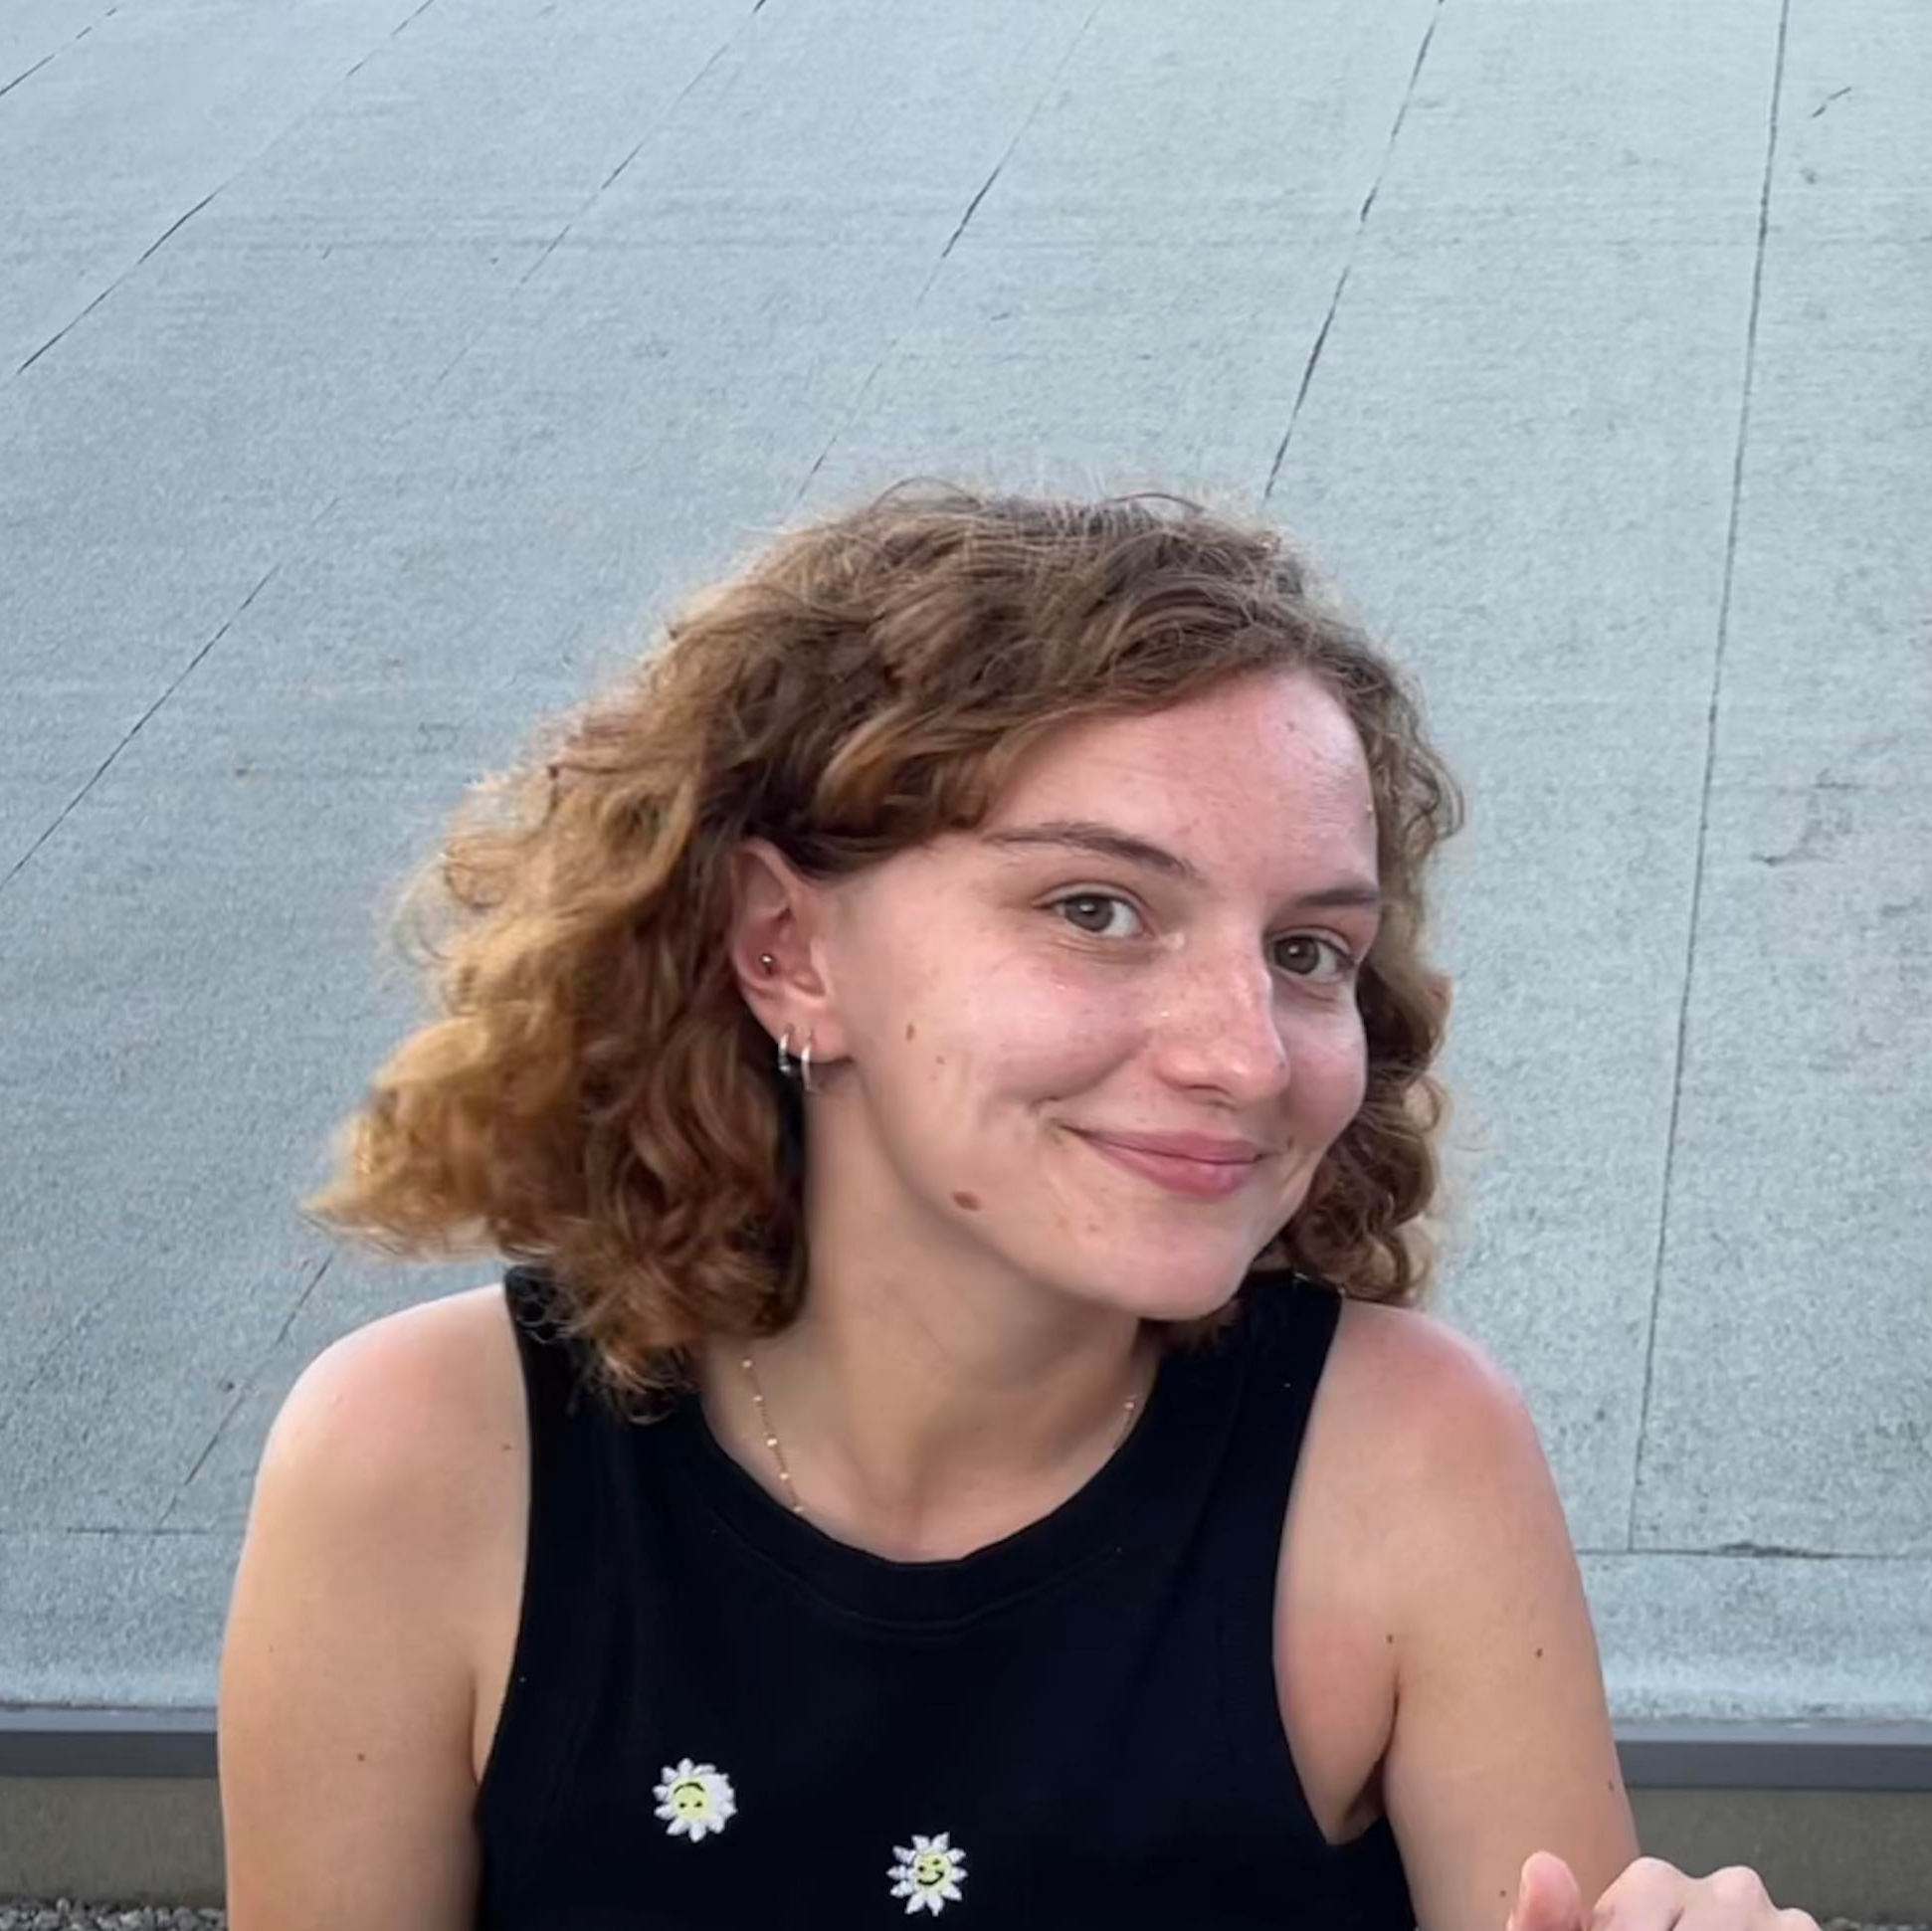
\includegraphics[height = 2.5cm]{Figures/lucie.png} & 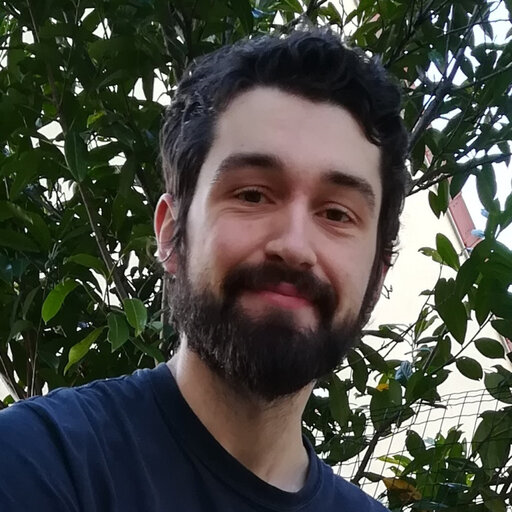
\includegraphics[height = 2.5cm]{Figures/corto.png} 	\end{tabular} \end{tabular} \vspace{-0.3cm}}
	\institute[]{Funded by ANR PaVeDyS \vspace{-0.3cm}}
	\setbeamertemplate{navigation symbols}{}
	\addtobeamertemplate{title page}{}{\begin{center}{To be published at FoSSaCS'24}\end{center}}
%	
%	
\begin{frame}
	\titlepage
\end{frame}	

\begin{frame}
	\tableofcontents
\end{frame}

\section{Introduction of the model}


\begin{frame}{Broadcast networks}
	\centering
	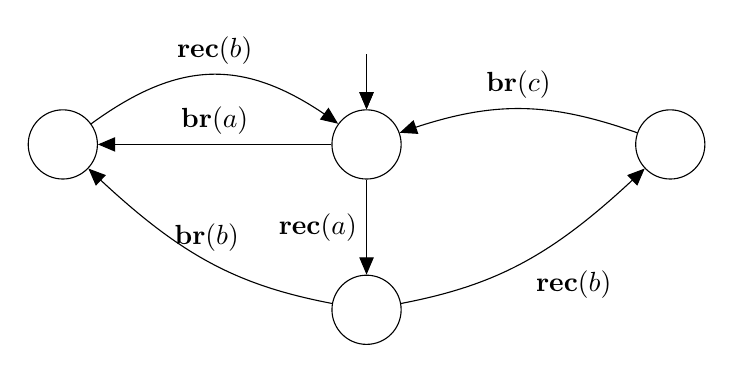
\begin{tikzpicture}[xscale=0.5,node distance=2.1cm,auto,>= triangle
	45]
	\tikzstyle{initial}= [initial by arrow,initial text=,initial
	distance=.7cm, initial above]
	%	\tikzstyle{accepting}= [accepting by arrow,accepting text=,accepting
	%	distance=.7cm,accepting where =right]
	
	\node[state,initial, minimum width=0.1pt] (0) at (0,0) {};
	\node[state] [left of=0, xshift=-50] (x) {};
	\node[state] [below of=0] (y) {};
	\node[state] [right of=0, xshift=50] (z) {};
	
\path[->, bend left=20] (x) edge node[above] {$\mathbf{rec}(b)$} (0);
	
	
	\path[->, bend left=10] 	
	(y) edge node[above] {$\mathbf{br}(b)$} (x)
	;
	
	\path[->] 	
	(0) edge node[left] {$\mathbf{rec}(a)$} (y)
	;
	
	\path[->](0) edge node[above] {$\mathbf{br}(a)$} (x);
	
	\path[->, bend right=10] 	
	(y) edge node[below right] {$\mathbf{rec}(b)$} (z)
	(z) edge node[above] {$\mathbf{br}(c)$} (0)
	;
\end{tikzpicture}
\end{frame}


\begin{frame}{Broadcast networks}
	\centering
	\hspace{-4cm}
\resizebox{5cm}{2.2cm}{
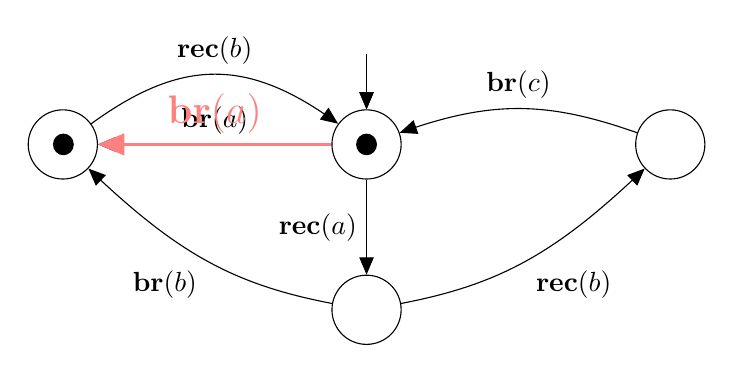
\begin{tikzpicture}[xscale=0.5,node distance=2.1cm,auto,>= triangle
	45]
	\tikzstyle{initial}= [initial by arrow,initial text=,initial
	distance=.7cm, initial above]
	%	\tikzstyle{accepting}= [accepting by arrow,accepting text=,accepting
	%	distance=.7cm,accepting where =right]
	
	\node[state,initial, minimum width=0.1pt] (0) at (0,0) {};
	\node[state] [left of=0, xshift=-50] (x) {};
	\node[state] [below of=0] (y) {};
	\node[state] [right of=0, xshift=50] (z) {};
	
	\onslide<1>{\draw[fill=black] (0,0) ellipse (0.25 and 0.13);}
	\onslide<2->{\draw[fill=black] (-7.7,0) ellipse (0.25 and 0.13);}
	
	\path[->, bend left=10] 	
	(y) edge node[below left] {$\mathbf{br}(b)$} (x)
	;
	
	\path[->, bend left=20] (x) edge node[above] {$\mathbf{rec}(b)$} (0);
	
	
	\path[->] 	
	(0) edge node[left] {$\mathbf{rec}(a)$} (y)
	;
	
	\onslide<1,3->{\path[->](0) edge node[above] {$\mathbf{br}(a)$} (x);}
	\onslide<2>{\path[->, very thick, red!50] (0) edge node[above] {\Large $\mathbf{br}(a)$} (x);}
	
	\path[->, bend right=10] 	
	(y) edge node[below right] {$\mathbf{rec}(b)$} (z)
	(z) edge node[above] {$\mathbf{br}(c)$} (0)
	;
\end{tikzpicture}
}

\hspace{4cm}
\resizebox{5cm}{2.2cm}{
	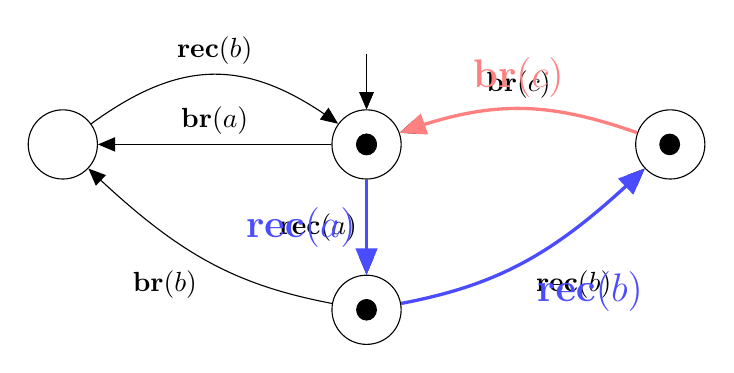
\begin{tikzpicture}[xscale=0.5,node distance=2.1cm,auto,>= triangle
		45]
		\tikzstyle{initial}= [initial by arrow,initial text=,initial
		distance=.7cm, initial above]
		%	\tikzstyle{accepting}= [accepting by arrow,accepting text=,accepting
		%	distance=.7cm,accepting where =right]
		
		\node[state,initial, minimum width=0.1pt] (0) at (0,0) {};
		\node[state] [left of=0, xshift=-50] (x) {};
		\node[state] [below of=0] (y) {};
		\node[state] [right of=0, xshift=50] (z) {};
		
		
		\onslide<2>{\draw[fill=black] (0,-2.1) ellipse (0.25 and 0.13);}
		\onslide<3>{\draw[fill=black] (7.7,0) ellipse (0.25 and 0.13);}
		\onslide<1>{\draw[fill=black] (0,0) ellipse (0.25 and 0.13);}
		\onslide<4>{\draw[fill=black] (0,0) ellipse (0.25 and 0.13);}
		
\path[->, bend left=20] (x) edge node[above] {$\mathbf{rec}(b)$} (0);
		
			\onslide<1-4>{\path[->,bend left=10](y) edge node[below left] {$\mathbf{br}(b)$} (x);}
		
		\onslide<1-2,4>{\path[->,bend right=10](y) edge node[below right] {$\mathbf{rec}(b)$} (z);}
		\onslide<3>{\path[->, very thick,bend right=10, blue!70] (y) edge node[below right] {\Large $\mathbf{rec}(b)$} (z);}
		
		\onslide<1-3>{\path[->,bend right=10](z) edge node[above] {$\mathbf{br}(c)$} (0);}
		\onslide<4>{\path[->, very thick,bend right=10, red!50] (z) edge node[above] {\Large $\mathbf{br}(c)$} (0);}
		
		\path[->] 	
		(0) edge node[above] {$\mathbf{br}(a)$} (x)
		;
		
		\onslide<1,3->{\path[->](0) edge node[left] {$\mathbf{rec}(a)$} (y);}
		\onslide<2>{\path[->, very thick, blue!70] (0) edge node[left] {\Large $\mathbf{rec}(a)$} (y);}
		;
	\end{tikzpicture}
}

\hspace{-4cm}
\resizebox{5cm}{2.2cm}{
	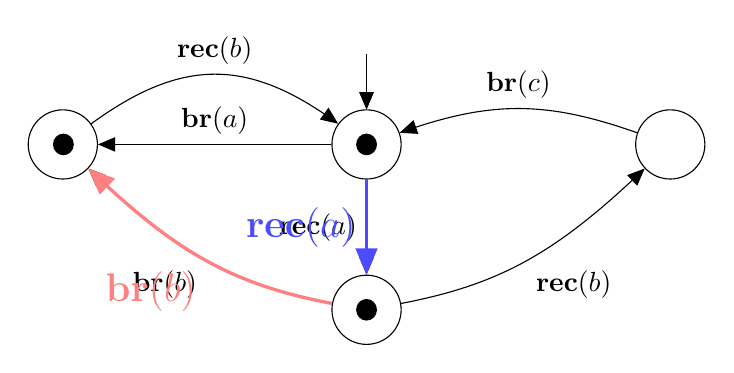
\begin{tikzpicture}[xscale=0.5,node distance=2.1cm,auto,>= triangle
		45]
		\tikzstyle{initial}= [initial by arrow,initial text=,initial
		distance=.7cm, initial above]
		%	\tikzstyle{accepting}= [accepting by arrow,accepting text=,accepting
		%	distance=.7cm,accepting where =right]
		
		\node[state,initial, minimum width=0.1pt] (0) at (0,0) {};
		\node[state] [left of=0, xshift=-50] (x) {};
		\node[state] [below of=0] (y) {};
		\node[state] [right of=0, xshift=50] (z) {};
		
		\onslide<1>{\draw[fill=black] (0,0) ellipse (0.25 and 0.13);}
		\onslide<2>{\draw[fill=black] (0,-2.1) ellipse (0.25 and 0.13);}
		\onslide<3->{\draw[fill=black] (-7.7,0) ellipse (0.25 and 0.13);}

		
		\path[->] 	
		(0) edge node[above] {$\mathbf{br}(a)$} (x)
		;
\path[->, bend left=20] (x) edge node[above] {$\mathbf{rec}(b)$} (0);
		
		
		\onslide<1,3->{\path[->](0) edge node[left] {$\mathbf{rec}(a)$} (y);}
		\onslide<2>{\path[->, very thick, blue!70] (0) edge node[left] {\Large $\mathbf{rec}(a)$} (y);}
		
		\onslide<1-2,4>{\path[->,bend left=10](y) edge node[below left] {$\mathbf{br}(b)$} (x);}
		\onslide<3>{\path[->, very thick,bend left=10, red!50] (y) edge node[below left] {\Large $\mathbf{br}(b)$} (x);}
		
		
		\path[->, bend right=10] 	
		(y) edge node[below right] {$\mathbf{rec}(b)$} (z)
		(z) edge node[above] {$\mathbf{br}(c)$} (0)
		;
	\end{tikzpicture}
}
\end{frame}

\begin{frame}{Broadcast Networks}
	\begin{block}{Definition\footnotemark}
		(Reconfigurable) Broadcast Network = $(Q, \messages, \Delta, q_0)$ with $\Delta \subseteq Q\times \{\mathbf{br}(m), \mathbf{rec}(m) \mid m \in \messages\} \times Q$.
	\end{block}
	
	\pause
	
	\begin{itemize}
		\item Arbitrarily many agents at the start
		
		\item One step = an agent broadcasts a message $m$,\\ some (arbitrary subset of) other agents receive it.
	\end{itemize}
	
	\pause 
	
	\begin{block}{Problems}
%		\vspace{0.3cm}
		{\COVER}: Is there a run in which \textbf{an} agent reaches $q_f$?
%		\vspace{0.3cm}
		
		{\TARGET}: Is there a run in which \textbf{all agents} reach $q_f$ \textbf{simultaneously}?
	\end{block}
	
	\onslide<3->
	Both problems are decidable in PTIME\footnote[1]{Delzanno, Sangnier, Zavattaro, CONCUR'10}\footnote<3>{Fournier, PhD thesis, 2015}.
\end{frame}

\begin{frame}{Adding registers}
	
	Each agent now has local \emph{registers} $\reg_1, \ldots, \reg_r$, containing values in $\mathbb{N}$.\vspace{0.3cm}\pause
	\begin{center}
	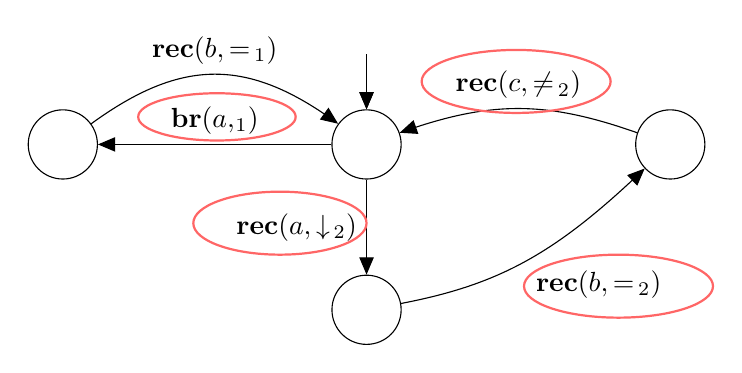
\begin{tikzpicture}[xscale=0.5,node distance=2.1cm,auto,>= triangle
	45]
	\tikzstyle{initial}= [initial by arrow,initial text=,initial
	distance=.7cm, initial above]
	%	\tikzstyle{accepting}= [accepting by arrow,accepting text=,accepting
	%	distance=.7cm,accepting where =right]
	
	\node[state,initial, minimum width=0.1pt] (0) at (0,0) {};
	\node[state] [left of=0, xshift=-50] (x) {};
	\node[state] [below of=0] (y) {};
	\node[state] [right of=0, xshift=50] (z) {};
	
	\path[->, bend left=20] (x) edge node[above] {$\mathbf{rec}(b, =\reg_1)$} (0);
	
%	\path[->, bend left=10] 	
%	(y) edge node[above] {$\mathbf{br}(b)$} (x)
%	;
	
	\path[->] 	
	(0) edge node[left] {$\mathbf{rec}(a, \downarrow \reg_2)$} (y)
	;
	
	\path[->](0) edge node[above] {$\mathbf{br}(a, \reg_1)$} (x);
	
	\path[->, bend right=10] 	
	(y) edge node[below right] {$\mathbf{rec}(b, = \reg_2)$} (z)
	(z) edge node[above] {$\mathbf{rec}(c, \neq \reg_2)$} (0)
	;
	
	\onslide<2>
	{
	\draw[color=red!60,thick] (-3.8,0.35) ellipse (2 and 0.3);
	}
	\onslide<3>
	{
		\draw[color=red!60,thick] (-2.2,-1) ellipse (2.2 and 0.4);
	}
	
	\onslide<4>
	{
		\draw[color=red!60,thick] (6.4,-1.8) ellipse (2.4 and 0.4);
	}
	
	\onslide<5>
	{
		\draw[color=red!60,thick] (3.8,0.8) ellipse (2.4 and 0.4);
	}
\end{tikzpicture}
	\end{center}
\end{frame}

\begin{frame}{Broadcast Networks of Register Automata (BNRA)\footnote{Delzanno, Sangnier, Traverso, RP'13}}
	Each agent now has local \emph{registers} $\reg_1, \ldots, \reg_r$, containing values in $\mathbb{N}$.
	\pause
	\textbf{Initially, all registers of all agents contain distinct values.}
	
	\pause
	\vspace{0.2cm}
	A message is a pair $(m, v) \in \messages \times \mathbb{N}$.
	An agent can:
	\begin{itemize}
		\item Broadcast a message symbol along with a register value: $\mathbf{br}(m, r_i)$\vspace{0.3cm}\pause
		
%		\item Test equality between its registers $\mathbf{loc}(r_i, r_j, =), \mathbf{loc}(r_i, r_j, \neq)$\pause
		
		\item Receive a message of a given symbol $m$: $\mathbf{rec}(m, \mathsf{op})$, with $\mathsf{op}$ one of the following:
		\begin{itemize}
			\item store the value in register $\reg_i$: $\downarrow \reg_i$,
			
			\item test it for equality with register $\reg_i$: $= \reg_i, \neq \reg_i$
			
			\item or discard the received value: $*$.
		\end{itemize}   
	\end{itemize}

	\pause
	This model was first defined in \footnotemark[3], where the authors prove that this model is undecidable if several values can be appended to the same message. They also wrongly claimed that, with one value per message (our model), coverability is decidable in \textsc{Pspace}.
\end{frame}

\begin{frame}{Things we can do}
	
	We can check that messages received come from the same agent.
	Here a word in $a \, b \, a^* \, c$ must be received with all messages having the same value: 
	\vspace{1cm}


	\centering
	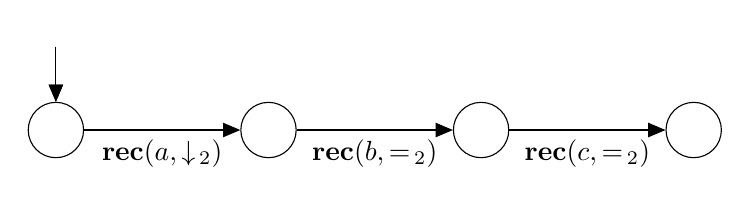
\begin{tikzpicture}[xscale=0.5,node distance=2.7cm,auto, AUT style,>= triangle
	45]
	\tikzstyle{initial}= [initial by arrow,initial text=,initial
	distance=.7cm, initial above]
	%	\tikzstyle{accepting}= [accepting by arrow,accepting text=,accepting
	%	distance=.7cm,accepting where =right]
	
	\node[state, initial, minimum width=0.1pt] (0) at (0,0) {};
	\node[state] [right of=0] (y) {};
	\node[state] [right of=y] (z) {};
	\node [state, right of = z] (s) {};
	
	
	%	\path[->, bend left=10] 	
	%	(y) edge node[above] {$\mathbf{br}(b)$} (x)
	%	;
	
	% \path[->, loop above] (z) edge node[above] {$\rec(a, =\reg_2)$} (z);
	
	\path[->] 	
	(0) edge node[below] {$\mathbf{rec}(a, \downarrow \reg_2)$} (y)
	(y) edge node[below] {$\mathbf{rec}(b, = \reg_2)$} (z)
	(z) edge node[below] {$\mathbf{rec}(c, = \reg_2)$} (s)
	;
	
\end{tikzpicture}
\end{frame}

\begin{frame}{Things we can do}
	We can check that a sequence of messages we sent was received. \\
	Here the top branch sends $a \, b$, the bottom branch receives $a \, b$ and sends an acknowledgement. 
	\vspace{0.5cm}

		\centering
		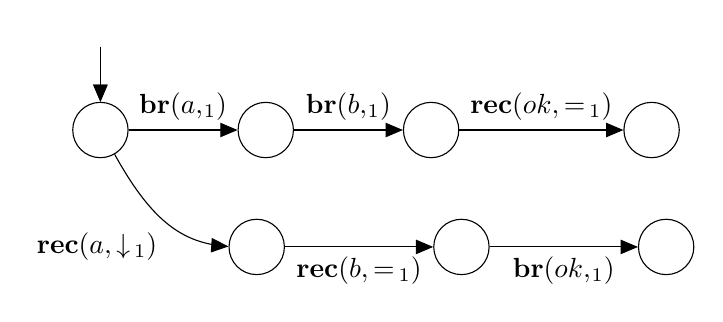
\begin{tikzpicture}[xscale=0.5,node distance=2.1cm,auto, AUT style,>= triangle
	45]
	\tikzstyle{initial}= [initial by arrow,initial text=,initial
	distance=.7cm, initial above]
	%	\tikzstyle{accepting}= [accepting by arrow,accepting text=,accepting
	%	distance=.7cm,accepting where =right]
	
	\node[state, initial, minimum width=0.1pt] (0) at (0,0) {};
	\node[state] [right of=0] (x) {};
	\node[state] [right of=x] (y) {};
	\node[state] [right of=y, xshift=0.7cm] (z) {};
	
	\node[state] [below right of=0, xshift=0.5cm] (x') {};
	\node[state] [right of=x', xshift=0.5cm] (y') {};
	\node[state] [right of=y',xshift=0.5cm] (z') {};
	
	
	%	\path[->, bend left=10] 	
	%	(y) edge node[above] {$\mathbf{br}(b)$} (x)
	%	;
	
	
	\path[->] 	
	(0) edge node[above] {$\mathbf{br}(a, \reg_1)$} (x)
	(x) edge node[above] {$\mathbf{br}(b, \reg_1)$} (y)
	(y) edge node[above] {$\mathbf{rec}(ok, = \reg_1)$} (z)
	(x') edge node[below] {$\mathbf{rec}(b, = \reg_1)$} (y')
	(y') edge node[below] {$\mathbf{br}(ok, \reg_1)$} (z')
	;
	
	\path[->, bend right=20] (0) edge node[below left] {$\mathbf{rec}(a, \downarrow \reg_1)$} (x');
	
\end{tikzpicture}
\end{frame}

\begin{frame}{Parameterized verification principles}
	
	\begin{block}{Our parameterized problems}
%		\vspace{0.3cm}
		{\COVER}: Is there \emph{a number of agents} $n$, a run over $n$ agents in which \textbf{an agent} reaches $q_f$?
%		\vspace{0.3cm}
		
		{\TARGET}: Is there \emph{a number of agents} $n$, a run over $n$ agents in which \textbf{all agents} reach $q_f$ \textbf{simultaneously}?
	\end{block}
	
	\pause

	\begin{itemize}
		\item Unlimited supply of agents.
		
		\item For {\COVER}, we can add as many agents as we need at no cost. 
	\end{itemize}
	
	\pause
	
	\begin{block}{Copycat principle}
		Given a run $\rho$, we can construct a run made of many copies of $\rho$ running in parallel.
	\end{block}
	
	\pause 

	\begin{block}{Main theorem}
		{\COVER} is decidable for BNRA.
	\end{block}
	
\end{frame}







\section{Decidability of \COVER for signature BNRA}


\begin{frame}{Signature BNRA}
	\begin{block}{Signature BNRA}
		An agent never modifies its first register, and only broadcasts with the value of its first signature.
		
		Other registers are used to store and compare values received.
	\end{block}
	The first register acts as an identity with which agents sign their messages. 
	
	\vspace{-0.4cm}
	\begin{center}
		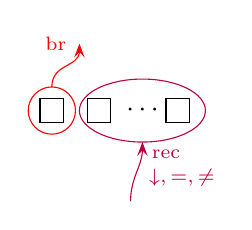
\begin{tikzpicture}
			\draw[red] (0.15,0.15) circle (0.3); 
			%		\node at (-0.2, -0.2) {\scriptsize\color{red} id};
			\node at (0.2, 1) {\scriptsize\color{red} br};
			\draw[purple] (1.3,0.15) ellipse (0.8 and 0.4);
			\node at (1.6, -0.4) {\scriptsize\color{purple} rec};
			\node at (1.8, -0.7) {\scriptsize\color{purple} $\downarrow, =, \neq$};
			
			\draw (0,0) rectangle (0.3,0.3);
			\draw (0.6,0) rectangle (0.9,0.3);
			\node at (1.3,0.15) {$\cdots$};
			\draw (1.6,0) rectangle (1.9,0.3);
			
			\draw[red, arrows = {-Stealth[length=5pt, inset=2pt]}] (0.15, 0.45) .. controls +(0,0.3) and +(0,-0.3) .. (0.5, 1); 
			\draw[purple, arrows = {-Stealth[length=5pt, inset=2pt]}] (1.15, -1) .. controls +(0,0.3) and +(0,-0.3) .. (1.3, -0.25); 
		\end{tikzpicture}
	\end{center}
	
	\pause
	\textbf{\small Messages received with the same value come from the same agent.}
\end{frame}




% \begin{frame}{Towards a tree abstraction}
% Assume that there is a valid run $\rho$ for \COVER. 
% \begin{block}{Observation 1}
% If agent $a$ broadcasts to agents $b$ and $c$, we can make copy agent $a$ so that $b$ and $c$ receive messages from distinct agents. 
% \end{block}
% We can modify $\rho$ so that each agent sends messages to one single agent.
% \pause

% \begin{block}{Observation 2}
% If $a$ broadcasts $m_1$ to $b$ then $b$ broadcasts $m_2$ to $a$, we can make a copy $a'$ of $a$ that broadcasts to $b$ and then stops; $a' \to b \to a$.
% \end{block}
% More generally, we can guarantee that the graph of ``who sends messages to whom'' has no cycle: it's a tree (or a forest) !
% \end{frame}
	

\begin{frame}{Tree witnesses for \COVER}
	
	\centering
	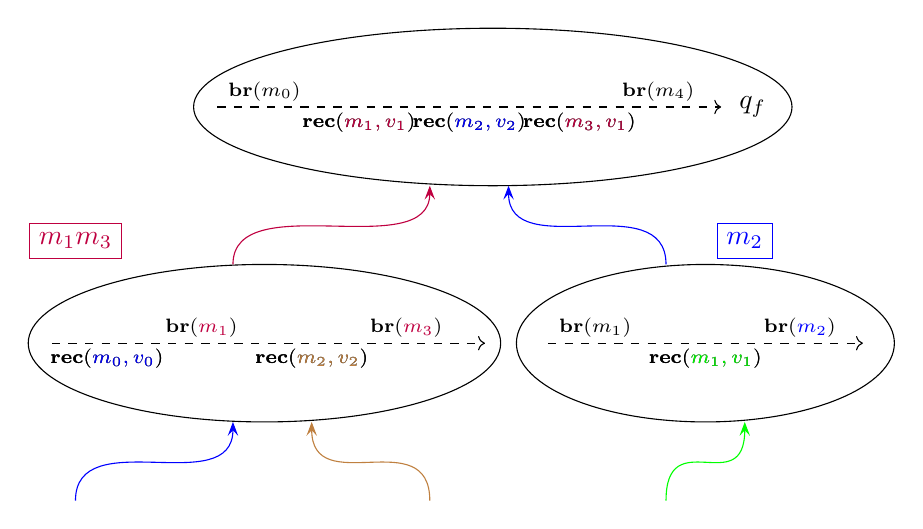
\begin{tikzpicture}
	
	\onslide<1-> 
	{
	\draw[->, dashed] (-0.2,0) -- (6.2,0);
	\node at (6.6,0) (qf) {$q_f$};
	\node (0) at (0.4,0.2) {\scriptsize $\br(m_0)$};
	\onslide<1>
	{
	\node (1) at (1.6,-0.2) {\scriptsize $\rec(m_1, v_1)$};
	\node (2) at (3,-0.2) {\scriptsize $\rec(m_2, v_2)$};
	\node (3) at (4.4,-0.2) {\scriptsize $\rec(m_3, v_1)$};
}
	\onslide<2->
	{
	\node (1) at (1.6,-0.2) {\scriptsize $\rec(\color{purple}m_1, v_1\color{black})$};
	\node (2) at (3,-0.2) {\scriptsize $\rec(\color{blue} m_2, v_2\color{black})$};
	\node (3) at (4.4,-0.2) {\scriptsize $\rec(\color{purple}m_3, v_1\color{black})$};
	}
	\node (4) at (5.4,0.2) {\scriptsize $\br(m_4)$};
	}
	
	
	
	\onslide<3-> 
	{
		\draw[->, dashed] (-2.3,-3) -- (3.2,-3);
		\node (0') at (-0.4,-2.8) {\scriptsize $\br(\color{purple}m_1\color{black})$};
		\node (1') at (-1.6,-3.2) {\scriptsize $\rec(m_0, v_0)$};
		\node (2') at (1,-3.2) {\scriptsize $\rec(m_2, v_2)$};
		\node (3') at (2.2,-2.8) {\scriptsize $\br(\color{purple}m_3\color{black})$};
	}
	
		\onslide<3-> 
	{
		\draw[->, dashed] (4,-3) -- (8,-3);
		\node (0'') at (4.6,-2.8) {\scriptsize $\br(\color{black}m_1\color{black})$};
		\node (2'') at (6,-3.2) {\scriptsize $\rec(m_1, v_1)$};
		\node (3'') at (7.2,-2.8) {\scriptsize $\br(\color{blue}m_2\color{black})$};
	}
	
	\onslide<4->
	{
		
		\draw (3.3,0) ellipse (3.8 and 1);
		\draw (0.4,-3) ellipse (3 and 1);
		\draw (6,-3) ellipse (2.4 and 1);
	\draw[purple, arrows = {-Stealth[length=5pt, inset=2pt]}] (0, -2) .. controls +(0,1) and +(0,-1) .. (2.5, -1); 
	\draw[blue, arrows = {-Stealth[length=5pt, inset=2pt]}] (5.5, -2) .. controls +(0,1) and +(0,-1) .. (3.5, -1);  
	
	\node[draw, purple] (Tp) at (-2,-1.7) {$m_1m_3$};
	\node[draw, blue] (Tb) at (6.5,-1.7) {$m_2$};
	% \node[draw, orange] (Tb) at (7,0) {$m$};
%	\draw[purple, arrows = {-Stealth[length=5pt, inset=2pt]}] (3.6, -1.7) .. controls +(0,1) and +(0,-1) .. (5.5, -0.4);
	}
	
	\onslide<5->
	{
		\draw[blue, arrows = {-Stealth[length=5pt, inset=2pt]}] (-2, -5) .. controls +(0,1) and +(0,-1) .. (0, -4); 
		\draw[brown, arrows = {-Stealth[length=5pt, inset=2pt]}] (2.5, -5) .. controls +(0,1) and +(0,-1) .. (1, -4);  
		\draw[green, arrows = {-Stealth[length=5pt, inset=2pt]}] (5.5, -5) .. controls +(0,1) and +(0,-1) .. (6.5, -4);  

		\node (1') at (-1.6,-3.2) {\scriptsize $\rec(\color{blue}m_0, v_0\color{black})$};
		\node (2') at (1,-3.2) {\scriptsize $\rec(\color{brown}m_2, v_2\color{black})$};
		\node (2'') at (6,-3.2) {\scriptsize $\rec(\color{green}m_1, v_1\color{black})$};
		
		%	\draw[purple, arrows = {-Stealth[length=5pt, inset=2pt]}] (3.6, -1.7) .. controls +(0,1) and +(0,-1) .. (5.5, -0.4);
	}
\end{tikzpicture}
	
\end{frame}

\begin{frame}{Tree witnesses for \COVER}
	\begin{center}
	\resizebox{!}{4.5cm}{
	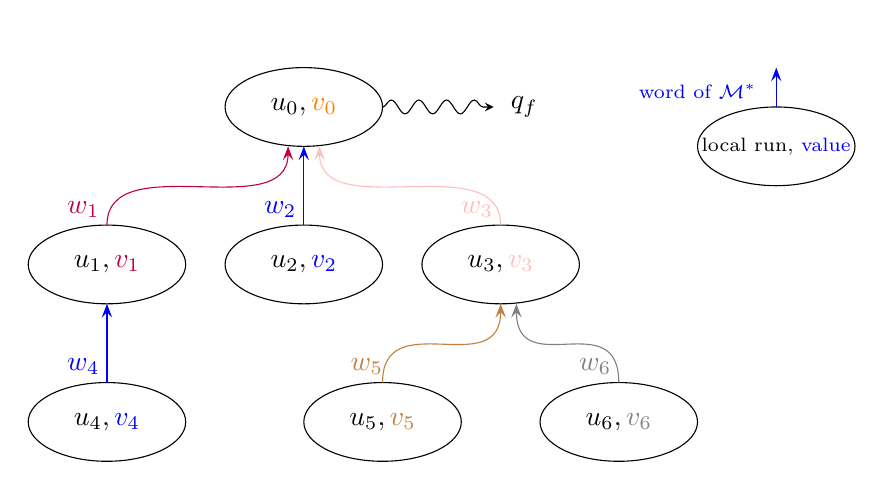
\begin{tikzpicture}
	
	\draw (1,0) ellipse (1 and 0.5);
	\node (u1) at (1,0) {$u_0,\color{orange} v_0$};
	
	\draw (-1.5,-2) ellipse (1 and 0.5);
	\node (u2) at (-1.5,-2) {$u_1, \color{purple} v_1$};
	
	\draw (1,-2) ellipse (1 and 0.5);
	\node (u3) at (1,-2) {$u_2, \color{blue} v_2$};
	
	\draw (3.5,-2) ellipse (1 and 0.5);
	\node (u4) at (3.5,-2) {$u_3, \color{pink} v_3$};
	
	\draw (2,-4) ellipse (1 and 0.5);
	\node (u6) at (2,-4) {$u_5, \color{brown}v_5$};
	
	\draw (-1.5,-4) ellipse (1 and 0.5);
	\node (u5) at (-1.5,-4) {$u_4, \color{blue}v_4$};
	
	\draw (5,-4) ellipse (1 and 0.5);
	\node (u7) at (5,-4) {$u_6, \color{gray}v_6$};
	
	
	\node (2) at (-1.8,-1.3) {\color{purple}$w_1$};
	\node (3) at (0.7,-1.3) {\color{blue}$w_2$};
	\node (4) at (3.2,-1.3) {\color{pink}$w_3$};
	\node (5) at (-1.8,-3.3) {\color{blue}$w_4$};
	\node (6) at (1.8,-3.3) {\color{brown}$w_5$};
	\node (7) at (4.7,-3.3) {\color{gray}$w_6$};
	\node (qf) at (3.8,0) {$q_f$};
	\draw[-stealth, decorate, decoration = snake] (2,0) -- (3.41,0);	
	

	\draw[blue, arrows = {-Stealth[length=5pt, inset=2pt]}] (-1.5, -3.5) .. controls +(0,1) and +(0,-1) .. (-1.5, -2.5); 
	
	
	\draw[brown, arrows = {-Stealth[length=5pt, inset=2pt]}] (2, -3.5) .. controls +(0,1) and +(0,-1) .. (3.5, -2.5);  
	\draw[gray, arrows = {-Stealth[length=5pt, inset=2pt]}] (5, -3.5) .. controls +(0,1) and +(0,-1) .. (3.7, -2.5); 
	
	\draw[blue, arrows = {-Stealth[length=5pt, inset=2pt]}] (1, -1.5) .. controls +(0,1) and +(0,-1) .. (1, -0.5); 
	\draw[purple, arrows = {-Stealth[length=5pt, inset=2pt]}] (-1.5, -1.5) .. controls +(0,1) and +(0,-1) .. (0.8, -0.5);  
	\draw[pink, arrows = {-Stealth[length=5pt, inset=2pt]}] (3.5, -1.5) .. controls +(0,1) and +(0,-1) .. (1.2, -0.5); 
	
	\begin{scope}[yshift = -1cm]
	\draw (7, 0.5) ellipse (1 and 0.5);
	\node (legend) at (7,0.5) {\scriptsize local run, \color{blue} value};
	\draw[blue, arrows = {-Stealth[length=5pt, inset=2pt]}] (7, 1) .. controls +(0,1) and +(0,-1) .. (7, 1.5); 
	\node (8) at (6, 1.2) {\color{blue}\scriptsize word of $\messages^*$};
	\end{scope}
\end{tikzpicture}
	}
	\end{center}
\pause

\begin{block}{Lemma}
There is a tree witness if and only if the instance of \COVER is positive.  
\end{block}
For decidability, we need to bound the size of well-chosen tree witnesses.
\end{frame}

\begin{frame}{Branch reduction}
	
	\begin{block}{Lemma}
		If a node labelled $w$ has a descendant labelled $w'$ with $w$ a subword of $w'$ (written $w \preceq w'$) then the tree can be shortened.
	\end{block}
	\begin{center}
	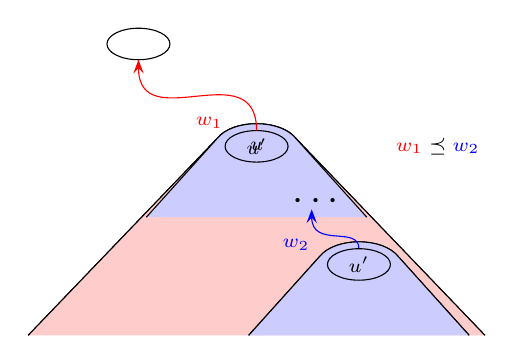
\begin{tikzpicture}
	
	\tikzset{every node/.style = {font = \scriptsize}}
	\onslide<2>
	{
		\draw (-0.4, -3.4) -- (2, -0.9) .. controls +(0.2,0.25) and +(-0.2,0.25) .. (3, -0.9) -- (5.4, -3.4); 
		\draw[fill=red!20] (-0.4, -3.4) -- (2, -0.9) .. controls +(0.2,0.25) and +(-0.2,0.25) .. (3, -0.9) -- (5.4, -3.4); 
		
		\draw (2.4, -3.4) -- (3.3, -2.4) .. controls +(0.2,0.25) and +(-0.2,0.25) .. (4.3, -2.4) -- (5.2, -3.4); 
		\draw[fill=blue!20] (2.4, -3.4) -- (3.3, -2.4) .. controls +(0.2,0.25) and +(-0.2,0.25) .. (4.3, -2.4) -- (5.2, -3.4); 
	}
	
	\onslide<3->
	{
%		\draw (-0.8, -3.8) -- (2, -0.9) .. controls +(0.2,0.25) and +(-0.2,0.25) .. (3, -0.9) -- (5.8, -3.8); 
		\draw[fill=blue!20] (1.1, -1.9) -- (2, -0.9) .. controls +(0.2,0.25) and +(-0.2,0.25) .. (3, -0.9) -- (3.9, -1.9); 
%		
%		\draw (2, -3.8) -- (3.3, -2.4) .. controls +(0.2,0.25) and +(-0.2,0.25) .. (4.3, -2.4) -- (5.6, -3.8); 
%		\draw[fill=blue!20] (2, -3.8) -- (3.3, -2.4) .. controls +(0.2,0.25) and +(-0.2,0.25) .. (4.3, -2.4) -- (5.6, -3.8); 
	}
	
	\draw (1,0.3) ellipse (0.4 and 0.2);
%	\node (u1) at (1,0) {$u_1,\color{orange} v_1$};
	
%	\draw (-1.5,-2) ellipse (1 and 0.5);
%	\node (u2) at (-1.5,-2) {$u_2, \color{purple} v_2$};
%	
%	\draw (1,-2) ellipse (1 and 0.5);
%	\node (u3) at (1,-2) {$u_3, \color{blue} v_3$};
%	
	\draw (2.5,-1) ellipse (0.4 and 0.2);
	\onslide<1-2>{\node (uv) at (2.5,-1) {\scriptsize $u$};}
	\onslide<3->{\node (uv) at (2.5,-1) {\scriptsize $u'$};}
%	\node (u4) at (3.5,-2) {$u_4, \color{pink} v_4$};
	
%	\node (u4) at (3.5,-2) {$u_4, \color{pink} v_4$};
%	
%	\draw (2,-4) ellipse (1 and 0.5);
%	\node (u6) at (2,-4) {$u_6, \color{brown}v_6$};
%	
%	\draw (-1.5,-4) ellipse (1 and 0.5);
%	\node (u5) at (-1.5,-4) {$u_5, \color{blue}v_5$};
%	
%	\draw (5,-4) ellipse (1 and 0.5);
%	\node (u7) at (5,-4) {$u_7, \color{gray}v_7$};
%	
	
%	\node (2) at (-1.8,-1.3) {\color{purple}$w_2$};
%	\node (3) at (0.7,-1.3) {\color{blue}$w_3$};
	\node (4) at (1.9,-0.7) {\color{red}$w_1$};
	\onslide<1-2>{\node (4) at (3,-2.25) {\color{blue}$w_2$};
		\draw[blue, arrows = {-Stealth[length=5pt, inset=2pt]}] (3.8, -2.3) .. controls +(0,0.3) and +(0,-0.5) .. (3.2, -1.8); 
		\node (dots) at (3.25, -1.7) {\Large$\cdots$};
		
		\draw (3.8,-2.5) ellipse (0.4 and 0.2);
		\node (u'v') at (3.8,-2.5) {\scriptsize $u'$};
	}
%	\node (5) at (-1.8,-3.3) {\color{blue}$w_5$};
%	\node (6) at (1.8,-3.3) {\color{brown}$w_6$};
%	\node (7) at (4.7,-3.3) {\color{gray}$w_7$};
%	\node (1) at (0.7,0.7) {\color{orange}$w_1$};	
	
	\node (txt) at (4.8,-1) {$\color{red} w_1 \color{black} \preceq \color{blue} w_2$};
%	
%	\draw[blue, arrows = {-Stealth[length=5pt, inset=2pt]}] (-1.5, -3.5) .. controls +(0,1) and +(0,-1) .. (-1.5, -2.5); 
%	
%	
%	\draw[brown, arrows = {-Stealth[length=5pt, inset=2pt]}] (2, -3.5) .. controls +(0,1) and +(0,-1) .. (3.5, -2.5);  
%	\draw[gray, arrows = {-Stealth[length=5pt, inset=2pt]}] (5, -3.5) .. controls +(0,1) and +(0,-1) .. (3.7, -2.5); 
%	
%	\draw[blue, arrows = {-Stealth[length=5pt, inset=2pt]}] (1, -1.5) .. controls +(0,1) and +(0,-1) .. (1, -0.5); 
%	\draw[purple, arrows = {-Stealth[length=5pt, inset=2pt]}] (-1.5, -1.5) .. controls +(0,1) and +(0,-1) .. (0.8, -0.5);  
	\draw[red, arrows = {-Stealth[length=5pt, inset=2pt]}] (2.5, -0.8) .. controls +(0,1) and +(0,-1) .. (1, 0.1); 
	

	
	
\end{tikzpicture}
	\end{center}
	\pause \pause \pause
	\vspace{-1cm}
	
	After iterating this shortening procedure, we end up with a tree in which a node labelled $w$ has no descendant labelled $w' \succeq w$. 
\end{frame}


\begin{frame}{Well quasi-orders}
		 
		
		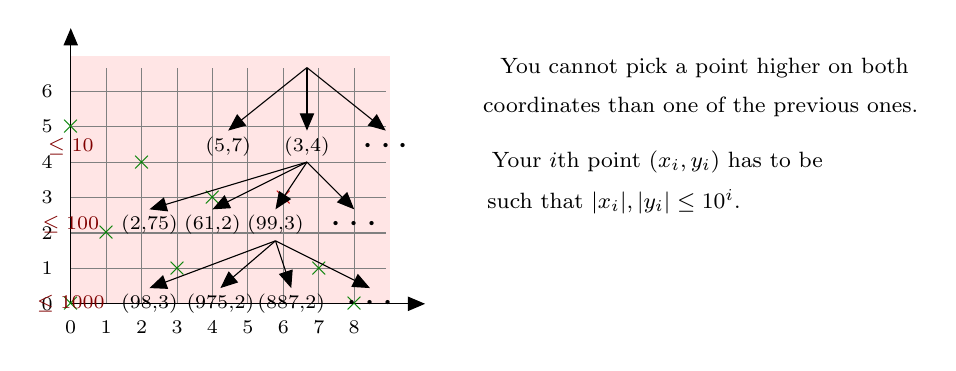
\begin{tikzpicture}[>= triangle 45]
	
\onslide<3-12>{\path [fill=red!10] (0.45*4, 0.45*3) rectangle (0.45*9, 0.45*7);}
\onslide<5-12>{\path [fill=red!10] (0.45*2, 0.45*4) rectangle (0.45*9, 0.45*7);}
\onslide<6-12>{\path [fill=red!10] (0.45*7, 0.45*1) rectangle (0.45*9, 0.45*7);}
\onslide<7-12>{\path [fill=red!10] (0.45*0, 0.45*5) rectangle (0.45*9, 0.45*7);}
\onslide<8-12>{\path [fill=red!10] (0.45*8, 0.45*0) rectangle (0.45*9, 0.45*7);}
\onslide<9-12>{\path [fill=red!10] (0.45*3, 0.45*1) rectangle (0.45*9, 0.45*7);}
\onslide<10-12>{\path [fill=red!10] (0.45*1, 0.45*2) rectangle (0.45*9, 0.45*7);}
\onslide<11-12>{\path [fill=red!10] (0.45*0, 0.45*0) rectangle (0.45*9, 0.45*7);}

\onslide<1-12>{
\draw[gray, step = 0.45] (0,0) grid (4,3);
\draw[->] (0,0) -- (4.5,0);
\draw[->] (0,0) -- (0,3.5);



\node (0) at (0*0.45,-0.3) {\scriptsize $0$};
\node (1) at (1*0.45,-0.3) {\scriptsize $1$};
\node (2) at (2*0.45,-0.3) {\scriptsize $2$};
\node (3) at (3*0.45,-0.3) {\scriptsize $3$};
\node (4) at (4*0.45,-0.3) {\scriptsize $4$};
\node (5) at (5*0.45,-0.3) {\scriptsize $5$};
\node (6) at (6*0.45,-0.3) {\scriptsize $6$};
\node (7) at (7*0.45,-0.3) {\scriptsize $7$};
\node (8) at (8*0.45,-0.3) {\scriptsize $8$};

\node (0) at (-0.3,0*0.45) {\scriptsize $0$};
\node (0) at (-0.3,1*0.45) {\scriptsize $1$};
\node (0) at (-0.3,2*0.45) {\scriptsize $2$};
\node (0) at (-0.3,3*0.45) {\scriptsize $3$};
\node (0) at (-0.3,4*0.45) {\scriptsize $4$};
\node (0) at (-0.3,5*0.45) {\scriptsize $5$};
\node (0) at (-0.3,6*0.45) {\scriptsize $6$};
}

\onslide<2-12> {\node[green!50!black] (0) at (0.45*4, 0.45*3) {$\times$};}
\onslide<4> {\node[red!80!black] (0) at (0.45*6, 0.45*3) {$\times$};}
\onslide<5-12> {\node[green!50!black] (0) at (0.45*2, 0.45*4) {$\times$};}
\onslide<6-12> {\node[green!50!black] (0) at (0.45*7, 0.45*1) {$\times$};}
\onslide<7-12> {\node[green!50!black] (0) at (0.45*0, 0.45*5) {$\times$};}
\onslide<8-12> {\node[green!50!black] (0) at (0.45*8, 0.45*0) {$\times$};}
\onslide<9-12> {\node[green!50!black] (0) at (0.45*3, 0.45*1) {$\times$};}
\onslide<10-12> {\node[green!50!black] (0) at (0.45*1, 0.45*2) {$\times$};}
\onslide<11-12> {\node[green!50!black] (0) at (0.45*0, 0.45*0) {$\times$};}

\onslide<3->{
\node (txt1) at (8, 3) {\footnotesize $\blacktriangleright$ You cannot pick a point higher on both} ;
\node (txt2) at (8, 2.5) {\footnotesize coordinates than one of the previous ones.} ;
}

\onslide<12->{
\node (txt1) at (7.4, 1.8) {\footnotesize $\blacktriangleright$ Your $i$th point $(x_i, y_i)$ has to be } ;
\node (txt2) at (6.9, 1.3) {\footnotesize such that $|x_i|, |y_i| \leq 10^i$.} ;
}

	\onslide<13->{
	\node (11) at (2,2) {\scriptsize(5,7)} ;
	\node (11) at (3,2) {\scriptsize(3,4)} ;
	\node (11) at (4,2) {\Large $\cdots$} ;
	
	\node (leq) at (0, 2) {\color{red!50!black}\scriptsize$\leq 10$};
	}

	\onslide<14->{
	\node (21) at (1,1) {\scriptsize(2,75)} ;
	\node (21) at (1.8,1) {\scriptsize(61,2)} ;
	\node (21) at (2.6,1) {\scriptsize(99,3)} ;
	\node (21) at (3.6,1) {\Large $\cdots$} ;
	\node (leq) at (0, 1) {\color{red!50!black}\scriptsize$\leq 100$};
	}

\onslide<15->{	
		\node (21) at (1,0) {\scriptsize(98,3)} ;
	\node (21) at (1.9,0) {\scriptsize(975,2)} ;
	\node (21) at (2.8,0) {\scriptsize(887,2)} ;
	\node (21) at (3.8,0) {\Large $\cdots$} ;
	\node (leq) at (0, 0) {\color{red!50!black}\scriptsize$\leq 1000$};
	}

\onslide<13-> {
	\draw[->] (3,3) -- (2,2.2);
	\draw[->] (3,3) -- (3,2.2);
	\draw[->] (3,3) -- (4,2.2);
}
\onslide<14-> {
	\draw[->] (3,1.8) -- (1,1.2);
	\draw[->] (3,1.8) -- (1.8,1.2);
	\draw[->] (3,1.8) -- (2.6,1.2);
	\draw[->] (3,1.8) -- (3.6,1.2);
}
\onslide<15->{
	\draw[->] (2.6,0.8) -- (1,0.2);
	\draw[->] (2.6,0.8) -- (1.9,0.2);
	\draw[->] (2.6,0.8) -- (2.8,0.2);
	\draw[->] (2.6,0.8) -- (3.8,0.2);
}

\end{tikzpicture}
		
		\onslide<1->{\onslide<2->{$(4,3)$}\onslide<4>{$\to {\color{red}(6,3)}$}\onslide<5->{\hspace{-1.35cm}$\to (2,4)$}\onslide<6->{$\to (7,1)$}\onslide<7->{$\to (0,5)$}\onslide<8->{$\to (8,0)$}\onslide<9->{$\to (3,1)$}\onslide<10->{$\to (1,2)$}\onslide<11->{$\to (0,0)$}}
		
		\onslide<12->
		This order on $\mathbb{N}^2$ is a \emph{well quasi-order} : every bad sequence is finite.

		\onslide<13->
			\begin{block}{Higman's lemma}
		For a finite alphabet $\Sigma$, the subword order $\preceq$ is a well quasi-order over $\Sigma^*$. In other words, there is no infinite bad sequence $w_0, w_1, w_2, \ldots$ in $\Sigma^*$, \emph{i.e.}, such that $w_i \npreceq w_j$ for all $i<j$.
	\end{block}
\end{frame}

\begin{frame}{Back to the trees}
If $q_f$ can be covered, then there is a witness of the execution of the form:
\begin{center}
\resizebox{!}{4cm}{
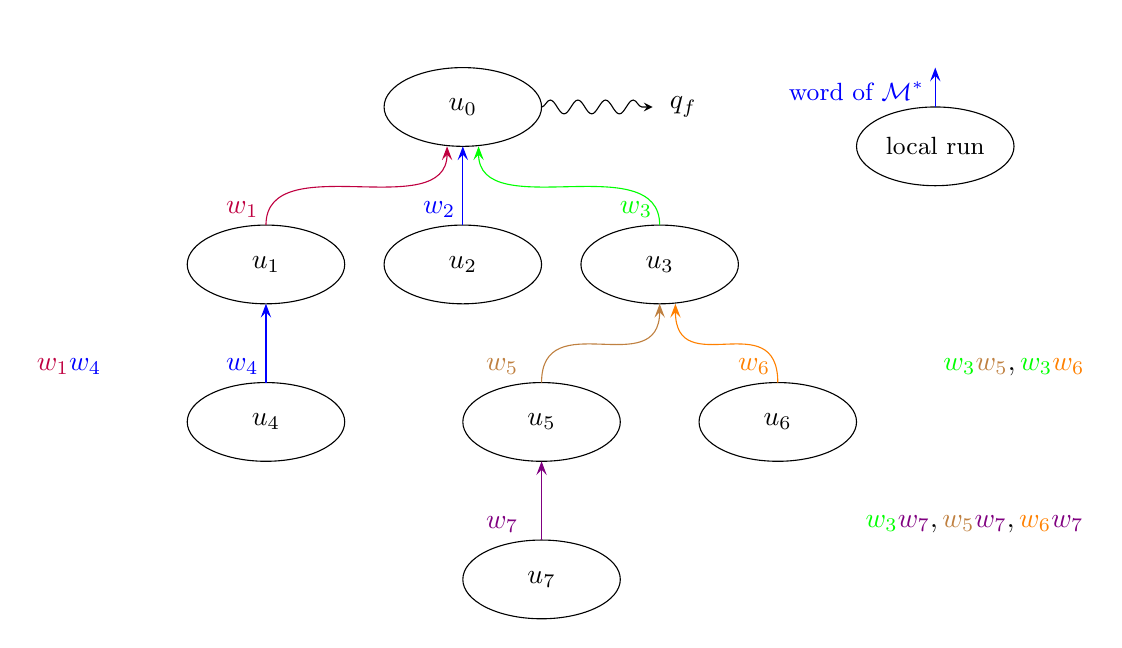
\begin{tikzpicture}
	
	\draw (1,0) ellipse (1 and 0.5);
	\node (u1) at (1,0) {$u_0$};
	
	\draw (-1.5,-2) ellipse (1 and 0.5);
	\node (u2) at (-1.5,-2) {$u_1$};
	
	\draw (1,-2) ellipse (1 and 0.5);
	\node (u3) at (1,-2) {$u_2$};
	
	\draw (3.5,-2) ellipse (1 and 0.5);
	\node (u4) at (3.5,-2) {$u_3$};
	
	\draw (2,-4) ellipse (1 and 0.5);
	\node (u6) at (2,-4) {$u_5$};

	\draw (2,-6) ellipse (1 and 0.5);
	\node (u7) at (2,-6) {$u_7$};
	
	\draw (-1.5,-4) ellipse (1 and 0.5);
	\node (u5) at (-1.5,-4) {$u_4$};
	
	\draw (5,-4) ellipse (1 and 0.5);
	\node (u7) at (5,-4) {$u_6$};
	
	
	\node (2) at (-1.8,-1.3) {\color{purple}$w_1$};
	\node (3) at (0.7,-1.3) {\color{blue}$w_2$};
	\node (4) at (3.2,-1.3) {\color{green}$w_3$};
	\node (5) at (-1.8,-3.3) {\color{blue}$w_4$};
	\node (6) at (1.5,-3.3) {\color{brown}$w_5$};
	\node (7) at (4.7,-3.3) {\color{orange}$w_6$};
	\node (8) at (1.5,-5.3) {\color{violet}$w_7$};
	\node (qf) at (3.8,0) {$q_f$};
	\draw[-stealth, decorate, decoration = snake] (2,0) -- (3.41,0);	
	

	\draw[blue, arrows = {-Stealth[length=5pt, inset=2pt]}] (-1.5, -3.5) .. controls +(0,1) and +(0,-1) .. (-1.5, -2.5); 
	
	
	\draw[brown, arrows = {-Stealth[length=5pt, inset=2pt]}] (2, -3.5) .. controls +(0,1) and +(0,-1) .. (3.5, -2.5);  
	\draw[orange, arrows = {-Stealth[length=5pt, inset=2pt]}] (5, -3.5) .. controls +(0,1) and +(0,-1) .. (3.7, -2.5); 
	
	\draw[blue, arrows = {-Stealth[length=5pt, inset=2pt]}] (1, -1.5) .. controls +(0,1) and +(0,-1) .. (1, -0.5); 
	\draw[purple, arrows = {-Stealth[length=5pt, inset=2pt]}] (-1.5, -1.5) .. controls +(0,1) and +(0,-1) .. (0.8, -0.5);  
	\draw[green, arrows = {-Stealth[length=5pt, inset=2pt]}] (3.5, -1.5) .. controls +(0,1) and +(0,-1) .. (1.2, -0.5); 

	\draw[violet, arrows = {-Stealth[length=5pt, inset=2pt]}] (2,-5.5) -- (2, -4.5);
	
	\begin{scope}[yshift = -1cm]
	\draw (7, 0.5) ellipse (1 and 0.5);
	\node (legend) at (7,0.5) {\small local run};
	\draw[blue, arrows = {-Stealth[length=5pt, inset=2pt]}] (7, 1) .. controls +(0,1) and +(0,-1) .. (7, 1.5); 
	\node (8) at (6, 1.2) {\color{blue}\small word of $\messages^*$};
	\end{scope}

	\node (ineqw4) at (-4,-3.3) {$\color{purple} w_1 \color{black} \npreceq \color{blue} w_4$};
	\node (ineqw56) at (8, -3.3) {$\color{green} w_3 \color{black} \npreceq \color{brown} w_5\color{black}, \color{green} w_3 \color{black} \npreceq \color{orange} w_6$}; 
	\node (ineqa7) at (7.5,-5.3) {$\color{green} w_3 \color{black} \npreceq \color{violet} w_7\color{black}, \color{brown} w_5 \color{black} \npreceq \color{violet} w_7\color{black}, \color{orange} w_6 \color{black} \npreceq \color{violet} w_7$};
\end{tikzpicture}
}
\end{center}

Every branch forms a bad sequence. Because $\preceq$ is a well quasi-order, we know that every branch of the tree is finite... 
\pause Not useful ! \\ We need a bound on the size of the tree, so that we can iterate over every possible such tree in finite time. 
\end{frame}

\begin{frame}{Bounds on the length of sequences}
	Obviously, there is no general bound on the length of a bad sequence: the sequence $m^k, m^{k-1}, \dots, m$ with $m \in \messages$ is a bad sequence of length $k$.  
	\pause
	However, there is a bound if we have some control on the size of the elements of the sequence:

	\begin{block}{Length function theorem\footnotemark}
	Given a finite alphabet $\Sigma$ and a computable function $F : \mathbb{N} \to \mathbb{N}$, there is a computable bound $B$ such that every sequence $(w_i)_{i \in \mathbb{N}}$ over $\Sigma$ such that
	\begin{itemize}
		\item $w_i \npreceq w_j$ for all $i<j$ (bad sequence) and
		\item $|w_i| \leq F(i)$ for all $i$
	\end{itemize}
has length at most $B$.
\end{block}
\footnotetext<2->{Schmitz, Schnoebelen, ICALP'11}
\end{frame}

\begin{frame}{Applying the length function theorem}
Consider a branch of a tree of minimal size: \vspace{0.2cm} 

\begin{center}
\resizebox{!}{4.5cm}{
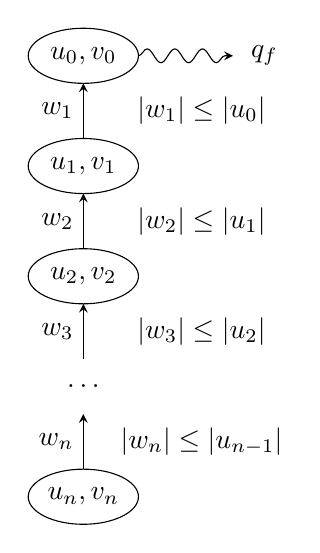
\begin{tikzpicture}[yscale = 0.7]
	\draw (0,2) ellipse (0.7 and 0.5);
	\node (u0) at (0,2) {$u_0, v_0$};

	\draw (0,0) ellipse (0.7 and 0.5);
	\node (u1) at (0,0) {$u_1, v_1$};
	
	\draw (0,-2) ellipse (0.7 and 0.5);
    \node (u2) at (0,-2) {$u_2, v_2$};

    \node (u3) at (0,-4) {$\dots$};

    \draw (0,-6) ellipse (0.7 and 0.5);
    \node (u4) at (0,-6) {$u_n, v_n$};

    \draw[-stealth] ($(u1)+(0,0.5)$) -- node[left] {$w_1$} ($(u0)-(0,0.5)$);
    \draw[-stealth] ($(u2)+(0,0.5)$) -- node[left] {$w_2$} ($(u1)-(0,0.5)$);
    \draw[-stealth] ($(u3)+(0,0.5)$) -- node[left] {$w_3$} ($(u2)-(0,0.5)$);
    \draw[-stealth] ($(u4)+(0,0.5)$) -- node[left] {$w_n$} ($(u3)-(0,0.5)$);
    \draw[-stealth, decorate, decoration = snake] (0.7,2) -- (1.9,2);
    \node (qf) at (2.3, 2) {$q_f$};

    \onslide<2->
    \node (w1bound) at (1.5,1) {$|w_1| \leq |u_0|$};
    \node (w2bound) at (1.5,-1) {$|w_2| \leq |u_1|$};
    \node (w3bound) at (1.5,-3) {$|w_3| \leq |u_2|$};
    \node (w4bound) at (1.5,-5) {$|w_n| \leq |u_{n-1}|$};


\end{tikzpicture}
}
\end{center}

\onslide<2->{
We need to bound the number of steps that an agent has to perform to perform a task: we need a function $f$ such that $|u_i| \leq f(|w_i|)$. }
\end{frame}

% \begin{frame}{Branch reduction}
% 	\begin{itemize}
% 		\item We can assume that a node labelled $w$ has no descendant labelled $w' \succeq w$.
% 		\pause 
% 		\item In order to bound the size of the tree, we need a bound on the growth of the size of the nodes.
% 	\end{itemize}

% 	\pause

% 	\begin{block}{Shortening long local runs} There exists a primitive recursive function $\varphi: \mathbb{N} \rightarrow \mathbb{N}$ such that, if an agent must broadcast $k$ messages, its local run does not need to have more than $k \, \varphi(|\mathcal{P}|)$ steps. 
% 	\end{block}
% 	$|\mathcal{P}|$: size of the protocol \\
% 	Proof by shortening arguments (a bit involved)
% \end{frame}


\begin{frame}{Bounding local runs}
	
	
	By induction on the number of \color{blue}\emph{active }\color{black} registers.
	
	Register $\reg_i$ is \emph{active} when some storing action $\downarrow \reg_i$ is performed. 
	\vspace{0.5cm}
	
	
	

	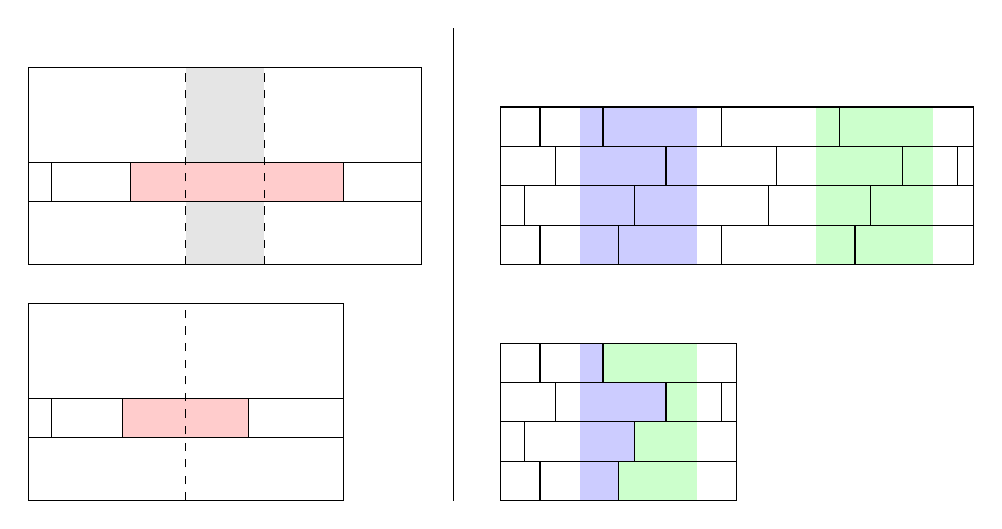
\begin{tikzpicture}
		\draw[white,fill=gray!20] (2,0) rectangle (3,0.8);
		\draw[white,fill=gray!20] (2,1.3) rectangle (3,2.5);
		
		\draw (0,0) rectangle (5,2.5);
		
		\draw (0,0.8) rectangle (5,1.3);
		
		\draw (0,0.8) rectangle (0.3,1.3);
		\draw (0,0.8) rectangle (1.3,1.3);
		\draw[fill=red!20] (1.3,0.8) rectangle (4,1.3);
		
		\draw[dashed] (2,0) -- (2,2.5);
		\draw[dashed] (3,0) -- (3,2.5);
		
		
		
		\draw (0,-3) rectangle (4,-0.5);
		
		\draw (0,-2.2) rectangle (4,-1.7);
		
		\draw (0,-2.2) rectangle (0.3,-1.7);
		\draw (0.3,-2.2) rectangle (1.3,-1.7);
		\draw[fill=red!20] (1.2,-2.2) rectangle (2.8,-1.7);
		
		\draw[dashed] (2,-3) -- (2,-0.5);
		
		\draw (5.4,-3) -- (5.4,3);
		
		
		\draw[white,fill=blue!20] (7,0) rectangle (8.5,2);
		\draw[white,fill=green!20] (10,0) rectangle (11.5,2);
		
		\draw (6,0) rectangle (12,2);
		
		\draw (6,0) rectangle (12,0.5);
		\draw (6,0) rectangle (12,1);
		\draw (6,0) rectangle (12,1.5);
		
		\draw (6,0) rectangle (6.5,0.5);
		\draw (6,0) rectangle (7.5,0.5);
		\draw (6,0) rectangle (8.8,0.5);
		\draw (6,0) rectangle (10.5,0.5);
		
		\draw (6,0.5) rectangle (6.3,1);
		\draw (6,0.5) rectangle (7.7,1);
		\draw (6,0.5) rectangle (9.4,1);
		\draw (6,0.5) rectangle (10.7,1);
		
		\draw (6,1) rectangle (6.7,1.5);
		\draw (6,1) rectangle (8.1,1.5);
		\draw (6,1) rectangle (9.5,1.5);
		\draw (6,1) rectangle (11.1,1.5);
		\draw (6,1) rectangle (11.8,1.5);
		
		\draw (6,1.5) rectangle (6.5,2);
		\draw (6,1.5) rectangle (7.3,2);
		\draw (6,1.5) rectangle (8.8,2);
		\draw (6,1.5) rectangle (10.3,2);
		
		
		\draw[white, fill=blue!20] (7,-3) rectangle (7.5,-2.5);
		\draw[white,fill=blue!20] (7,-2.5) rectangle (7.7,-2);
		\draw[white,fill=blue!20] (7,-2) rectangle (8.1,-1.5);
		\draw[white,fill=blue!20] (7,-1.5) rectangle (7.3,-1);
		
		\draw[white,fill=green!20] (7.5,-3) rectangle (8.5,-2.5);
		\draw[white,fill=green!20] (7.7,-2.5) rectangle (8.5,-2);
		\draw[white,fill=green!20] (8.1,-2) rectangle (8.5,-1.5);
		\draw[white,fill=green!20] (7.3,-1.5) rectangle (8.5,-1);
		
		
		
		\draw (6,-3) rectangle (9,-2.5);
		\draw (6,-3) rectangle (9,-2);
		\draw (6,-3) rectangle (9,-1.5);
		\draw (6,-3) rectangle (9,-1);
		
		\draw (6,-3) rectangle (6.5,-2.5);
		\draw (6,-3) rectangle (7.5,-2.5);
		
		\draw (6,-2.5) rectangle (6.3,-2);
		\draw (6,-2.5) rectangle (7.7,-2);
		
		\draw (6,-2) rectangle (6.7,-1.5);
		\draw (6,-2) rectangle (8.1,-1.5);
		\draw (6,-2) rectangle (8.8,-1.5);
		
		\draw (6,-1.5) rectangle (6.5,-1);
		\draw (6,-1.5) rectangle (7.3,-1);
		
	\end{tikzpicture}


\end{frame}

\begin{frame}{Bounding the tree}
	
	\begin{block}{Lemma}
		There is a function $\varphi$ such that if an agent has a local run between two local configurations, then it has one such local run of length $\leq \varphi(|\Delta|,r)$. 
	\end{block}
	
	$\Delta$: set of transitions \hspace{1cm} $r$: number of registers.
	
	\begin{block}{Corollary}
		If an agent has a local run that broadcasts $w$, then it has one such local run of length $\leq |w| \, \varphi(|\Delta|,r)$. 
	\end{block}
\end{frame}

\begin{frame}{Bounding the branches}
	\begin{center}
	\resizebox{!}{5cm}{
	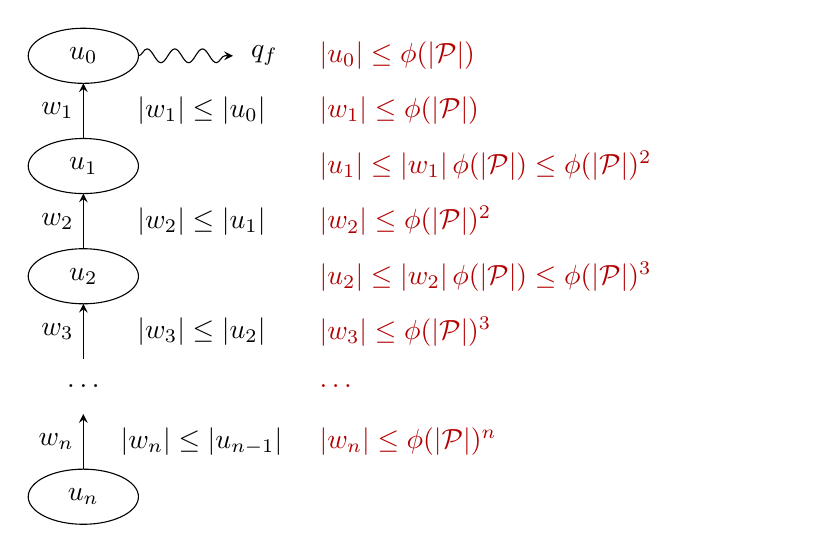
\begin{tikzpicture}[yscale = 0.7]
	\draw (0,2) ellipse (0.7 and 0.5);
	\node (u0) at (0,2) {$u_0$};

	\draw (0,0) ellipse (0.7 and 0.5);
	\node (u1) at (0,0) {$u_1$};
	
	\draw (0,-2) ellipse (0.7 and 0.5);
    \node (u2) at (0,-2) {$u_2$};

    \node (u3) at (0,-4) {$\dots$};

    \draw (0,-6) ellipse (0.7 and 0.5);
    \node (u4) at (0,-6) {$u_n$};

    \draw[-stealth] ($(u1)+(0,0.5)$) -- node[left] {$w_1$} ($(u0)-(0,0.5)$);
    \draw[-stealth] ($(u2)+(0,0.5)$) -- node[left] {$w_2$} ($(u1)-(0,0.5)$);
    \draw[-stealth] ($(u3)+(0,0.5)$) -- node[left] {$w_3$} ($(u2)-(0,0.5)$);
    \draw[-stealth] ($(u4)+(0,0.5)$) -- node[left] {$w_n$} ($(u3)-(0,0.5)$);
    \draw[-stealth, decorate, decoration = snake] (0.7,2) -- (1.9,2);
    \node (qf) at (2.3, 2) {$q_f$};
    \node (w1bound) at (1.5,1) {$|w_1| \leq |u_0|$};
    \node (w2bound) at (1.5,-1) {$|w_2| \leq |u_1|$};
    \node (w3bound) at (1.5,-3) {$|w_3| \leq |u_2|$};
    \node (w4bound) at (1.5,-5) {$|w_n| \leq |u_{n-1}|$};

    \onslide<2->
    \tikzset{every node/.style = {text = red!70!black, align = left, text width = 6cm}}
    \begin{scope}[xshift = 1cm]
    \node at (5,2) {$|u_0| \leq \phi(|\mathcal{P}|)$};
    \node at (5,1) {$|w_1| \leq \phi(|\mathcal{P}|)$};
    \node at (5,0) {$|u_1| \leq |w_1| \, \phi(|\mathcal{P}|) \leq \phi(|\mathcal{P}|)^2$};
    \node at (5,-1) {$|w_2| \leq \phi(|\mathcal{P}|)^2$};
    \node at (5,-2) {$|u_2| \leq  |w_2| \, \phi(|\mathcal{P}|) \leq \phi(|\mathcal{P}|)^3$};
    \node at (5,-3) {$|w_3| \leq \phi(|\mathcal{P}|)^3$};
    \node at (5,-4) {$\dots$};
    \node at (5,-5) {$|w_n| \leq \phi(|\mathcal{P}|)^n$};
    \end{scope}
    % \node at (5,-6) {$|u_n| \leq \phi(|\mathcal{P}|)^{n+1}$};
\end{tikzpicture}
	}
	\end{center}

	\onslide<3->{
	Length function theorem: we obtain a computable bound $B(|\Delta|, r)$ such that $n \leq B(|\Delta|, r)$: $B$ bounds the height of a witness tree for \COVER !
	}
\end{frame}


\begin{frame}{Decidability and complexity}
	\begin{block}{Bounds}
	We use the previous argument to bound (in well-chosen witness trees):
	\begin{itemize}
	\item the length of all branches,
	\item the size of every node,
	\item the maximal degree of the tree.
	\end{itemize}
	This bounds the total space needed to store such a tree.
	\end{block}
	\pause 

	We can enumerate all such trees in finite time, therefore
	
	\begin{block}{Theorem}
		The {\COVER} problem for \color{blue}signature \color{black} BNRA is decidable \onslide<3->{\color{red!70!black} and in $\mathbf{F}_{\omega^\omega}$.}
	\end{block} 
	\onslide<3->
	The length function theorem in fact gives us a bound for the height of our trees that is a function in hyper-Ackermannian class $\mathcal{F}_{\omega^\omega}$ of $|\Delta|$ and $r$. 
	% \onslide<4->{Can be extended to the non-signature case.} 
\end{frame}


\section{Decidability of \COVER in the general case}


\begin{frame}{General case}
	Agents can broadcast messages with values that they received before.
	\vspace{0.5cm}
	
	An agent $a$ now receives two types of messages:
	\begin{itemize}
		\item Messages with values that belonged to other agents initially.
		
		\item Messages with values that $a$ had initially, that it had broadcast and that someone else stored and broadcasts.  
	\end{itemize}
\end{frame}

\begin{frame}{Observation}
	
	An agent may do this:
	
	\[ \br(a, \reg_1) \, \br(b, \reg_1) \, \rec(c, =\reg_1)  \,\rec(d, =\reg_1) \, \rec(c, =\reg_1)\]
	\pause
	
	To witness that this is feasible, we must exhibit: 
	\begin{itemize}
		\item A run that, after receiving $(a, v) (b, v)$, broadcasts $(c,v)$, and
		
		\item A run that, after receiving $(a,v) (b,v) (c,v)^*$, broadcasts $(d,v)$.
	\end{itemize}
\vspace{0.5cm}

	\pause
	\textbf{We add \emph{contract} nodes labelled \fbox{$w \to m$} that witness a local run that, if it receives word $w$ with value $v$, can broadcast $(m,v)$.}
\end{frame}

\begin{frame}{Our new tree witnesses}
	
	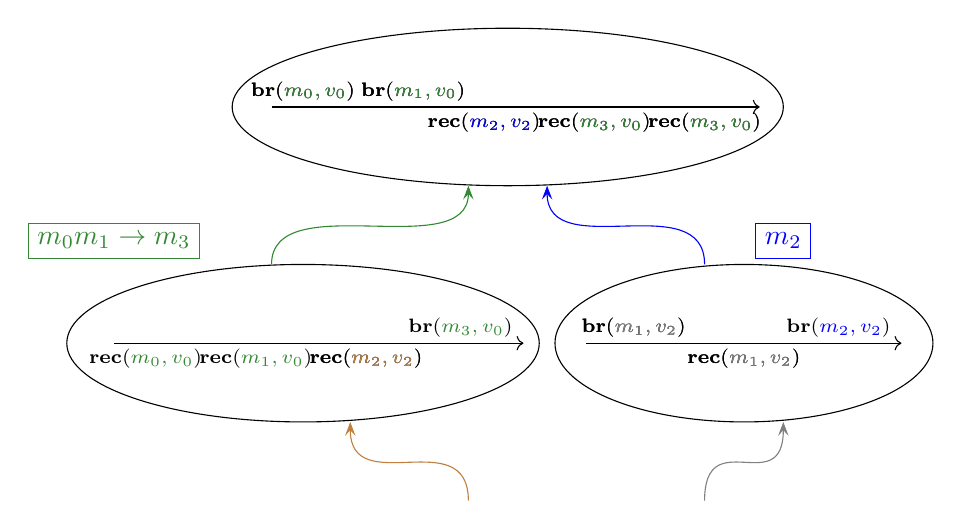
\begin{tikzpicture}
	
	\onslide<1-> 
	{
		\draw[->] (0,0) -- (6.2,0);
		\node (0) at (0.4,0.2) {\scriptsize $\br(m_0, v_0)$};
		\onslide<1>
		{
			\node (1) at (1.8,0.2) {\scriptsize $\br(m_1, v_0)$};
			\node (2) at (2.7,-0.2) {\scriptsize $\rec(m_2, v_2)$};
			\node (3) at (4.1,-0.2) {\scriptsize $\rec(m_3, v_0)$};
			\node (3) at (5.5,-0.2) {\scriptsize $\rec(m_3, v_0)$};
		}
		\onslide<2->
		{
			
			\node (0) at (0.4,0.2) {\scriptsize $\br(\color{DarkGreen}m_0, v_0\color{black})$};
			\node (1) at (1.8,0.2) {\scriptsize $\br(\color{DarkGreen}m_1, v_0\color{black})$};
			\node (2) at (2.7,-0.2) {\scriptsize $\rec(\color{blue} m_2, v_2\color{black})$};
			\node (3) at (4.1,-0.2) {\scriptsize $\rec(\color{DarkGreen}m_3, v_0\color{black})$};
			\node (4) at (5.5,-0.2) {\scriptsize $\rec(\color{DarkGreen}m_3, v_0\color{black})$};
		}
	}
	
	
	
	\onslide<3-> 
	{
		\draw[->] (-2,-3) -- (3.2,-3);
		\node (0') at (-0.2,-3.2) {\scriptsize $\rec(\color{DarkGreen}m_1, v_0\color{black})$};
		\node (1') at (-1.6,-3.2) {\scriptsize $\rec(\color{DarkGreen}m_0, v_0\color{black})$};
		\node (2') at (1.2,-3.2) {\scriptsize $\rec(m_2, v_2)$};
		\node (3') at (2.4,-2.8) {\scriptsize $\br(\color{DarkGreen}m_3, v_0\color{black})$};
	}
	
	\onslide<3-> 
	{
		\draw[->] (4,-3) -- (8,-3);
		\node (0'') at (4.6,-2.8) {\scriptsize $\br(\color{black}m_1, v_2\color{black})$};
		\node (2'') at (6,-3.2) {\scriptsize $\rec(m_1, v_2)$};
		\node (3'') at (7.2,-2.8) {\scriptsize $\br(\color{blue}m_2, v_2\color{black})$};
	}
	
	\onslide<4->
	{
		
		\draw (3,0) ellipse (3.5 and 1);
		\draw (0.4,-3) ellipse (3 and 1);
		\draw (6,-3) ellipse (2.4 and 1);
		\draw[DarkGreen, arrows = {-Stealth[length=5pt, inset=2pt]}] (0, -2) .. controls +(0,1) and +(0,-1) .. (2.5, -1); 
		\draw[blue, arrows = {-Stealth[length=5pt, inset=2pt]}] (5.5, -2) .. controls +(0,1) and +(0,-1) .. (3.5, -1);  
		
		\node[draw, DarkGreen] (Tp) at (-2,-1.7) {$m_0m_1 \to m_3 $};
		\node[draw, blue] (Tb) at (6.5,-1.7) {$m_2$};
		%	\draw[purple, arrows = {-Stealth[length=5pt, inset=2pt]}] (3.6, -1.7) .. controls +(0,1) and +(0,-1) .. (5.5, -0.4);
	}
	
	\onslide<5->
	{
%		\draw[blue, arrows = {-Stealth[length=5pt, inset=2pt]}] (-2, -5) .. controls +(0,1) and +(0,-1) .. (0, -4); 
		\draw[brown, arrows = {-Stealth[length=5pt, inset=2pt]}] (2.5, -5) .. controls +(0,1) and +(0,-1) .. (1, -4);  
		\draw[gray, arrows = {-Stealth[length=5pt, inset=2pt]}] (5.5, -5) .. controls +(0,1) and +(0,-1) .. (6.5, -4);  
		
%		\node (1') at (-1.6,-3.2) {\scriptsize $\rec(\color{blue}m_0, v_0\color{black})$};
		\node (2') at (1.2,-3.2) {\scriptsize $\rec(\color{brown}m_2, v_2\color{black})$};
		\node (2'') at (6,-3.2) {\scriptsize $\rec(\color{gray}m_1, v_2\color{black})$};
		\node (2'') at (4.6,-2.8) {\scriptsize $\br(\color{gray}m_1, v_2\color{black})$};
		
		%	\draw[purple, arrows = {-Stealth[length=5pt, inset=2pt]}] (3.6, -1.7) .. controls +(0,1) and +(0,-1) .. (5.5, -0.4);
	}
\end{tikzpicture}
	
\end{frame}


\begin{frame}{Branch reductions}
	\begin{columns}
		\begin{column}{0.5\textwidth}
			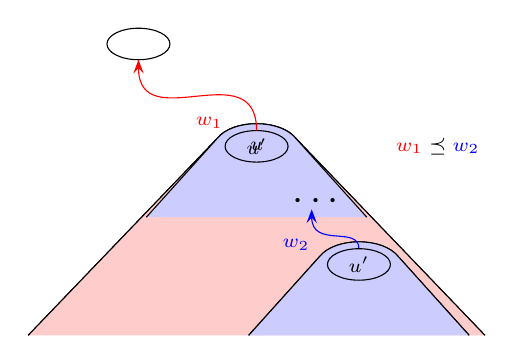
\begin{tikzpicture}
	
	\tikzset{every node/.style = {font = \scriptsize}}
	\onslide<2>
	{
		\draw (-0.4, -3.4) -- (2, -0.9) .. controls +(0.2,0.25) and +(-0.2,0.25) .. (3, -0.9) -- (5.4, -3.4); 
		\draw[fill=red!20] (-0.4, -3.4) -- (2, -0.9) .. controls +(0.2,0.25) and +(-0.2,0.25) .. (3, -0.9) -- (5.4, -3.4); 
		
		\draw (2.4, -3.4) -- (3.3, -2.4) .. controls +(0.2,0.25) and +(-0.2,0.25) .. (4.3, -2.4) -- (5.2, -3.4); 
		\draw[fill=blue!20] (2.4, -3.4) -- (3.3, -2.4) .. controls +(0.2,0.25) and +(-0.2,0.25) .. (4.3, -2.4) -- (5.2, -3.4); 
	}
	
	\onslide<3->
	{
%		\draw (-0.8, -3.8) -- (2, -0.9) .. controls +(0.2,0.25) and +(-0.2,0.25) .. (3, -0.9) -- (5.8, -3.8); 
		\draw[fill=blue!20] (1.1, -1.9) -- (2, -0.9) .. controls +(0.2,0.25) and +(-0.2,0.25) .. (3, -0.9) -- (3.9, -1.9); 
%		
%		\draw (2, -3.8) -- (3.3, -2.4) .. controls +(0.2,0.25) and +(-0.2,0.25) .. (4.3, -2.4) -- (5.6, -3.8); 
%		\draw[fill=blue!20] (2, -3.8) -- (3.3, -2.4) .. controls +(0.2,0.25) and +(-0.2,0.25) .. (4.3, -2.4) -- (5.6, -3.8); 
	}
	
	\draw (1,0.3) ellipse (0.4 and 0.2);
%	\node (u1) at (1,0) {$u_1,\color{orange} v_1$};
	
%	\draw (-1.5,-2) ellipse (1 and 0.5);
%	\node (u2) at (-1.5,-2) {$u_2, \color{purple} v_2$};
%	
%	\draw (1,-2) ellipse (1 and 0.5);
%	\node (u3) at (1,-2) {$u_3, \color{blue} v_3$};
%	
	\draw (2.5,-1) ellipse (0.4 and 0.2);
	\onslide<1-2>{\node (uv) at (2.5,-1) {\scriptsize $u$};}
	\onslide<3->{\node (uv) at (2.5,-1) {\scriptsize $u'$};}
%	\node (u4) at (3.5,-2) {$u_4, \color{pink} v_4$};
	
%	\node (u4) at (3.5,-2) {$u_4, \color{pink} v_4$};
%	
%	\draw (2,-4) ellipse (1 and 0.5);
%	\node (u6) at (2,-4) {$u_6, \color{brown}v_6$};
%	
%	\draw (-1.5,-4) ellipse (1 and 0.5);
%	\node (u5) at (-1.5,-4) {$u_5, \color{blue}v_5$};
%	
%	\draw (5,-4) ellipse (1 and 0.5);
%	\node (u7) at (5,-4) {$u_7, \color{gray}v_7$};
%	
	
%	\node (2) at (-1.8,-1.3) {\color{purple}$w_2$};
%	\node (3) at (0.7,-1.3) {\color{blue}$w_3$};
	\node (4) at (1.9,-0.7) {\color{red}$w_1$};
	\onslide<1-2>{\node (4) at (3,-2.25) {\color{blue}$w_2$};
		\draw[blue, arrows = {-Stealth[length=5pt, inset=2pt]}] (3.8, -2.3) .. controls +(0,0.3) and +(0,-0.5) .. (3.2, -1.8); 
		\node (dots) at (3.25, -1.7) {\Large$\cdots$};
		
		\draw (3.8,-2.5) ellipse (0.4 and 0.2);
		\node (u'v') at (3.8,-2.5) {\scriptsize $u'$};
	}
%	\node (5) at (-1.8,-3.3) {\color{blue}$w_5$};
%	\node (6) at (1.8,-3.3) {\color{brown}$w_6$};
%	\node (7) at (4.7,-3.3) {\color{gray}$w_7$};
%	\node (1) at (0.7,0.7) {\color{orange}$w_1$};	
	
	\node (txt) at (4.8,-1) {$\color{red} w_1 \color{black} \preceq \color{blue} w_2$};
%	
%	\draw[blue, arrows = {-Stealth[length=5pt, inset=2pt]}] (-1.5, -3.5) .. controls +(0,1) and +(0,-1) .. (-1.5, -2.5); 
%	
%	
%	\draw[brown, arrows = {-Stealth[length=5pt, inset=2pt]}] (2, -3.5) .. controls +(0,1) and +(0,-1) .. (3.5, -2.5);  
%	\draw[gray, arrows = {-Stealth[length=5pt, inset=2pt]}] (5, -3.5) .. controls +(0,1) and +(0,-1) .. (3.7, -2.5); 
%	
%	\draw[blue, arrows = {-Stealth[length=5pt, inset=2pt]}] (1, -1.5) .. controls +(0,1) and +(0,-1) .. (1, -0.5); 
%	\draw[purple, arrows = {-Stealth[length=5pt, inset=2pt]}] (-1.5, -1.5) .. controls +(0,1) and +(0,-1) .. (0.8, -0.5);  
	\draw[red, arrows = {-Stealth[length=5pt, inset=2pt]}] (2.5, -0.8) .. controls +(0,1) and +(0,-1) .. (1, 0.1); 
	

	
	
\end{tikzpicture}
		\end{column}
		
		\begin{column}{0.5\textwidth}
			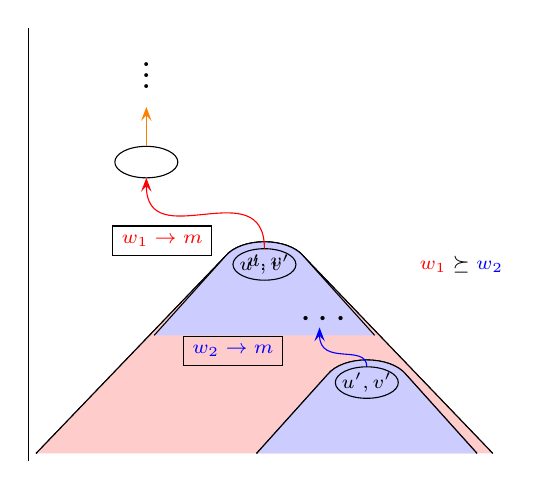
\begin{tikzpicture}
	\tikzset{every node/.style = {font = \scriptsize}}
	\draw (-0.5,-3.5) -- (-0.5,2);
	
	\onslide<2>
	{
		\draw (-0.4, -3.4) -- (2, -0.9) .. controls +(0.2,0.25) and +(-0.2,0.25) .. (3, -0.9) -- (5.4, -3.4); 
		\draw[fill=red!20] (-0.4, -3.4) -- (2, -0.9) .. controls +(0.2,0.25) and +(-0.2,0.25) .. (3, -0.9) -- (5.4, -3.4); 
		
		\draw (2.4, -3.4) -- (3.3, -2.4) .. controls +(0.2,0.25) and +(-0.2,0.25) .. (4.3, -2.4) -- (5.2, -3.4); 
		\draw[fill=blue!20] (2.4, -3.4) -- (3.3, -2.4) .. controls +(0.2,0.25) and +(-0.2,0.25) .. (4.3, -2.4) -- (5.2, -3.4); 
	}
	
	\onslide<3->
	{
		%		\draw (-0.8, -3.8) -- (2, -0.9) .. controls +(0.2,0.25) and +(-0.2,0.25) .. (3, -0.9) -- (5.8, -3.8); 
		\draw[fill=blue!20] (1.1, -1.9) -- (2, -0.9) .. controls +(0.2,0.25) and +(-0.2,0.25) .. (3, -0.9) -- (3.9, -1.9); 
		%		
		%		\draw (2, -3.8) -- (3.3, -2.4) .. controls +(0.2,0.25) and +(-0.2,0.25) .. (4.3, -2.4) -- (5.6, -3.8); 
		%		\draw[fill=blue!20] (2, -3.8) -- (3.3, -2.4) .. controls +(0.2,0.25) and +(-0.2,0.25) .. (4.3, -2.4) -- (5.6, -3.8); 
	}
	
	\draw (1,0.3) ellipse (0.4 and 0.2);
	%	\node (u1) at (1,0) {$u_1,\color{orange} v_1$};
	
	%	\draw (-1.5,-2) ellipse (1 and 0.5);
	%	\node (u2) at (-1.5,-2) {$u_2, \color{purple} v_2$};
	%	
	%	\draw (1,-2) ellipse (1 and 0.5);
	%	\node (u3) at (1,-2) {$u_3, \color{blue} v_3$};
	%	
	\draw (2.5,-1) ellipse (0.4 and 0.2);
	\onslide<1-2>{\node (uv) at (2.5,-1) {\scriptsize $u,v$};}
	\onslide<3->{\node (uv) at (2.5,-1) {\scriptsize $u',v'$};}
	%	\node (u4) at (3.5,-2) {$u_4, \color{pink} v_4$};
	
	%	\node (u4) at (3.5,-2) {$u_4, \color{pink} v_4$};
	%	
	%	\draw (2,-4) ellipse (1 and 0.5);
	%	\node (u6) at (2,-4) {$u_6, \color{brown}v_6$};
	%	
	%	\draw (-1.5,-4) ellipse (1 and 0.5);
	%	\node (u5) at (-1.5,-4) {$u_5, \color{blue}v_5$};
	%	
	%	\draw (5,-4) ellipse (1 and 0.5);
	%	\node (u7) at (5,-4) {$u_7, \color{gray}v_7$};
	%	
	
	%	\node (2) at (-1.8,-1.3) {\color{purple}$w_2$};
	%	\node (3) at (0.7,-1.3) {\color{blue}$w_3$};
	\node[draw] (4) at (1.2,-0.7) {\color{red}${w_1 \to m}$};
	\onslide<1-2>{\node[rectangle, draw] (4) at (2.1,-2.1) {\color{blue}$w_2 \to m$};
		\draw[blue, arrows = {-Stealth[length=5pt, inset=2pt]}] (3.8, -2.3) .. controls +(0,0.3) and +(0,-0.5) .. (3.2, -1.8); 
		\node (dots) at (3.25, -1.7) {\Large$\cdots$};
		
		\draw (3.8,-2.5) ellipse (0.4 and 0.2);
		\node (u'v') at (3.8,-2.5) {\scriptsize $u',v'$};
	}
	%	\node (5) at (-1.8,-3.3) {\color{blue}$w_5$};
	%	\node (6) at (1.8,-3.3) {\color{brown}$w_6$};
	%	\node (7) at (4.7,-3.3) {\color{gray}$w_7$};
	%	\node (1) at (0.7,0.7) {\color{orange}$w_1$};	
	
	\node (txt) at (5,-1) {$\color{red} w_1 \color{black} \succeq \color{blue} w_2$};
	% \node (txt) at (5,-1.5) {$\color{red} m \color{black} = \color{blue} m'$};
	
	\draw[orange, arrows = {-Stealth[length=5pt, inset=2pt]}] (1, 0.5) .. controls +(0,1) and +(0,-1) .. (1, 1); 
	%	
	%	\draw[blue, arrows = {-Stealth[length=5pt, inset=2pt]}] (-1.5, -3.5) .. controls +(0,1) and +(0,-1) .. (-1.5, -2.5); 
	%	
	%	
	%	\draw[brown, arrows = {-Stealth[length=5pt, inset=2pt]}] (2, -3.5) .. controls +(0,1) and +(0,-1) .. (3.5, -2.5);  
	%	\draw[gray, arrows = {-Stealth[length=5pt, inset=2pt]}] (5, -3.5) .. controls +(0,1) and +(0,-1) .. (3.7, -2.5); 
	%	
	%	\draw[blue, arrows = {-Stealth[length=5pt, inset=2pt]}] (1, -1.5) .. controls +(0,1) and +(0,-1) .. (1, -0.5); 
	%	\draw[purple, arrows = {-Stealth[length=5pt, inset=2pt]}] (-1.5, -1.5) .. controls +(0,1) and +(0,-1) .. (0.8, -0.5);  
	\draw[red, arrows = {-Stealth[length=5pt, inset=2pt]}] (2.5, -0.8) .. controls +(0,1) and +(0,-1) .. (1, 0.1); 
	
	
	\node (vdots) at (1, 1.5) {\Large$\vdots$};
	
	
\end{tikzpicture}
		\end{column}
	\end{columns}
	
\end{frame}

\begin{frame}{Things are more complicated than before}
	\begin{center}
	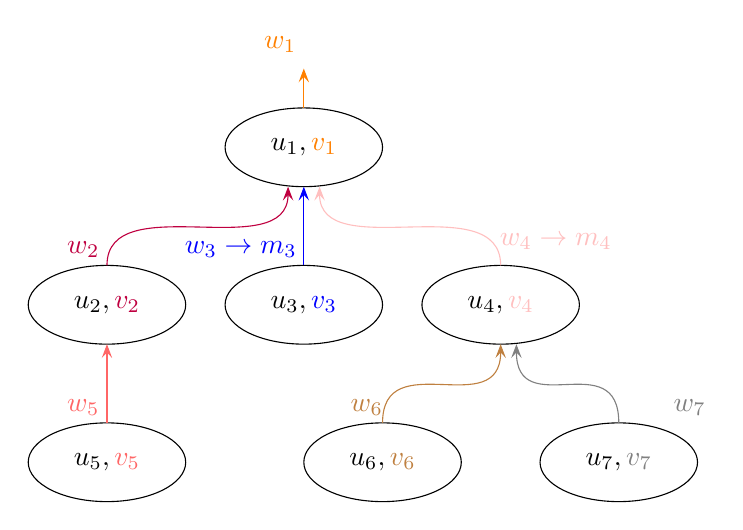
\begin{tikzpicture}
	
	\draw (1,0) ellipse (1 and 0.5);
	\node (u1) at (1,0) {$u_1,\color{orange} v_1$};
	
	\draw (-1.5,-2) ellipse (1 and 0.5);
	\node (u2) at (-1.5,-2) {$u_2, \color{purple} v_2$};
	
	\onslide<1>{
		\draw (1,-2) ellipse (1 and 0.5);
		\node (u3) at (1,-2) {$u_3, \color{blue} v_3$};
	}
	
	
	\onslide<1>
	{
		\draw (3.5,-2) ellipse (1 and 0.5);
		\node (u4) at (3.5,-2) {$u_4, \color{pink} v_4$};
	}

	
	\onslide<1>
	{
		\draw (2,-4) ellipse (1 and 0.5);
		\node (u6) at (2,-4) {$u_6, \color{brown}v_6$};
	}
	

	
	\draw (-1.5,-4) ellipse (1 and 0.5);
	\node (u5) at (-1.5,-4) {$u_5, \color{red!60}v_5$};
	
	\onslide<1>
	{
		\draw (5,-4) ellipse (1 and 0.5);
		\node (u7) at (5,-4) {$u_7, \color{gray}v_7$};
	}
	

	
	\node (2) at (-1.8,-1.3) {\color{purple}$w_2$};
	
	\onslide<1>
	{
		\node (7) at (5.9,-3.3) {\color{gray}$w_7$};
		\node (3) at (0.2,-1.3) {\color{blue}$w_3 \to m_3$};
		\node (4) at (4.2,-1.2) {\color{pink}$w_4 \to m_4$};
		\node (6) at (1.8,-3.3) {\color{brown}$w_6$};
	}
	\node (5) at (-1.8,-3.3) {\color{red!60}$w_5$};
	\node (1) at (0.7,1.3) {\color{orange}$w_1$};
	

	
	\draw[orange, arrows = {-Stealth[length=5pt, inset=2pt]}] (1, 0.5) .. controls +(0,1) and +(0,-1) .. (1, 1); 
	
	\draw[red!60, arrows = {-Stealth[length=5pt, inset=2pt]}] (-1.5, -3.5) .. controls +(0,1) and +(0,-1) .. (-1.5, -2.5); 
	
	\onslide<1>
	{
		\draw[brown, arrows = {-Stealth[length=5pt, inset=2pt]}] (2, -3.5) .. controls +(0,1) and +(0,-1) .. (3.5, -2.5);
	}

	
	
	\onslide<1>
	{  
		\draw[gray, arrows = {-Stealth[length=5pt, inset=2pt]}] (5, -3.5) .. controls +(0,1) and +(0,-1) .. (3.7, -2.5); 
	}
	

	\onslide<1>
	{
		\draw[blue, arrows = {-Stealth[length=5pt, inset=2pt]}] (1, -1.5) .. controls +(0,1) and +(0,-1) .. (1, -0.5); 
	}
	

	
	\draw[purple, arrows = {-Stealth[length=5pt, inset=2pt]}] (-1.5, -1.5) .. controls +(0,1) and +(0,-1) .. (0.8, -0.5);  
	
	\onslide<1>
	{
		\draw[pink, arrows = {-Stealth[length=5pt, inset=2pt]}] (3.5, -1.5) .. controls +(0,1) and +(0,-1) .. (1.2, -0.5); 
	}
	

	
\end{tikzpicture}
	\end{center}

	Problem: The number of messages that a node must broadcast now depends on its \fbox{$w \to m$} children, and not just on its father.
\end{frame}

\begin{frame}{Rearranging our trees}
	\centering
	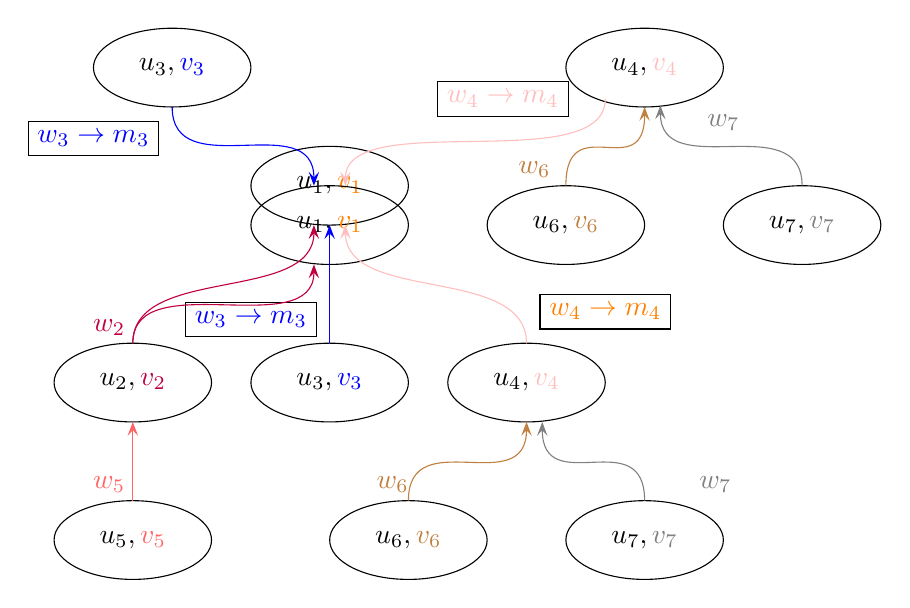
\begin{tikzpicture}
	
	\onslide<1>{
	\draw (1,0.5) ellipse (1 and 0.5);
	\node (u1) at (1,0.5) {$u_1,\color{orange} v_1$};
	}

	\onslide<2->{
	\draw (1,0) ellipse (1 and 0.5);
	\node (u1) at (1,0) {$u_1,\color{orange} v_1$};
	}
	
	\draw (-1.5,-2) ellipse (1 and 0.5);
	\node (u2) at (-1.5,-2) {$u_2, \color{purple} v_2$};
	
	\onslide<1>{
	\draw (1,-2) ellipse (1 and 0.5);
	\node (u3) at (1,-2) {$u_3, \color{blue} v_3$};
}

	\onslide<2->
	{
	\draw (-1,2) ellipse (1 and 0.5);
	\node (u3) at (-1,2) {$u_3, \color{blue} v_3$};
	}

	\onslide<1>
	{
	\draw (3.5,-2) ellipse (1 and 0.5);
	\node (u4) at (3.5,-2) {$u_4, \color{pink} v_4$};
}

	\onslide<2->
{
	\draw (5,2) ellipse (1 and 0.5);
	\node (u4) at (5,2) {$u_4, \color{pink} v_4$};
}

\onslide<1>
{
	\draw (2,-4) ellipse (1 and 0.5);
	\node (u6) at (2,-4) {$u_6, \color{brown}v_6$};
}

\onslide<2->
{
	\draw (4,0) ellipse (1 and 0.5);
	\node (u6) at (4,0) {$u_6, \color{brown}v_6$};
}

	
	\draw (-1.5,-4) ellipse (1 and 0.5);
	\node (u5) at (-1.5,-4) {$u_5, \color{red!60}v_5$};
	
	\onslide<1>
	{
	\draw (5,-4) ellipse (1 and 0.5);
	\node (u7) at (5,-4) {$u_7, \color{gray}v_7$};
}

	\onslide<2->
{
	\draw (7,0) ellipse (1 and 0.5);
	\node (u7) at (7,0) {$u_7, \color{gray}v_7$};
}

	
	\node (2) at (-1.8,-1.3) {\color{purple}$w_2$};
	
	\onslide<1>
	{
	\node (7) at (5.9,-3.3) {\color{gray}$w_7$};
	\node[draw] (3) at (0,-1.2) {\color{blue}$w_3 \to m_3$};
		\node[draw] (4) at (4.5,-1.1) {\color{orange}$w_4 \to m_4$};
	\node (6) at (1.8,-3.3) {\color{brown}$w_6$};
}
	\node (5) at (-1.8,-3.3) {\color{red!60}$w_5$};
	
		\onslide<2->
	{
		\node (7) at (6,1.3) {\color{gray}$w_7$};
		\node[draw] (3) at (-2,1.1) {\color{blue}$w_3 \to m_3$};
		\node[draw] (4) at (3.2,1.6) {\color{pink}$w_4 \to m_4$};
		\node (6) at (3.6,0.7) {\color{brown}$w_6$};
	}	
	 
	
	\draw[red!60, arrows = {-Stealth[length=5pt, inset=2pt]}] (-1.5, -3.5) .. controls +(0,1) and +(0,-1) .. (-1.5, -2.5); 
	
	\onslide<1>
	{
	\draw[brown, arrows = {-Stealth[length=5pt, inset=2pt]}] (2, -3.5) .. controls +(0,1) and +(0,-1) .. (3.5, -2.5);
}
		\onslide<2->
	{
		\draw[brown, arrows = {-Stealth[length=5pt, inset=2pt]}] (4, 0.5) .. controls +(0,1) and +(0,-1) .. (5, 1.5);
	}	
	
	
	\onslide<1>
	{  
	\draw[gray, arrows = {-Stealth[length=5pt, inset=2pt]}] (5, -3.5) .. controls +(0,1) and +(0,-1) .. (3.7, -2.5); 
}

	\onslide<2->
{  
	\draw[gray, arrows = {-Stealth[length=5pt, inset=2pt]}] (7, 0.5) .. controls +(0,1) and +(0,-1) .. (5.2, 1.52); 
}

	\onslide<1>
	{
	\draw[blue, arrows = {-Stealth[length=5pt, inset=2pt]}] (1, -1.5) .. controls +(0,1) and +(0,-1) .. (1, 0); 
	\draw[purple, arrows = {-Stealth[length=5pt, inset=2pt]}] (-1.5, -1.5) .. controls +(0,1) and +(0,-1) .. (0.8, 0);  
	
}

\onslide<2->
{
	\draw[blue, arrows = {-Stealth[length=5pt, inset=2pt]}] (-1, 1.5) .. controls +(0,-1) and +(0,1) .. (0.8, 0.5); 
	\draw[purple, arrows = {-Stealth[length=5pt, inset=2pt]}] (-1.5, -1.5) .. controls +(0,1) and +(0,-1) .. (0.8, -0.5);  
	
}
	
	
	\onslide<1>
	{
	\draw[pink, arrows = {-Stealth[length=5pt, inset=2pt]}] (3.5, -1.5) .. controls +(0,1) and +(0,-1) .. (1.2, 0); 
}

	\onslide<2->
{
	\draw[pink, arrows = {-Stealth[length=5pt, inset=2pt]}] (4.5, 1.6) .. controls +(0,-1) and +(0,1) .. (1.2, 0.5); 
}
	
\end{tikzpicture}
\end{frame}

\begin{frame}{Rearranging the tree}
	\begin{definition}
		The \emph{altitude} of a node is 
		
		\begin{itemize}
			\item 0 if it is the root
			
			\item its father's altitude $+1$ if it is labelled \fbox{$w \to m$}
		
			\item its father's altitude $-1$ if it is labelled $w$
		\end{itemize}
	\end{definition}
\end{frame}

\begin{frame}{Bounding the altitude}
	
	Let $A$ be the maximal altitude in the tree, we follow a branch reaching it. 
	
	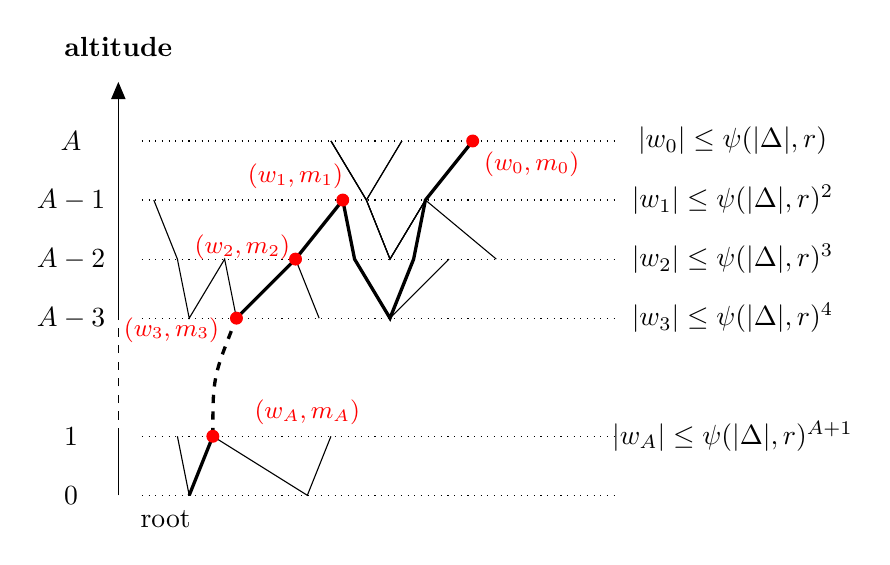
\begin{tikzpicture}[scale=1.5]
	
	\draw[dotted] (0,-0.5) -- (4,-0.5);
	\draw[dotted] (0,0) -- (4,0);
	\draw[dotted] (0,1) -- (4,1);
	\draw[dotted] (0,1.5) -- (4,1.5);
	\draw[dotted] (0,2) -- (4,2);
	\draw[dotted] (0,2.5) -- (4,2.5);
	
	\node at (-0.6,-0.5) {$0$};
	\node at (-0.6,0) {$1$};
	\node at (-0.6,1) {$A-3$};
	\node at (-0.6,1.5) {$A-2$};
	\node at (-0.6,2) {$A-1$};
	\node at (-0.6,2.5) {$A$};
	
	\onslide<4->
	{
		\node at (5,2.5) {$|w_0| \leq \psi(|\Delta|, r)$};	
	}
	
	\onslide<5->
	{
		\node at (5,2) {$|w_1| \leq \psi(|\Delta|, r)^2$};
		\node at (5,1.5) {$|w_2|  \leq \psi(|\Delta|, r)^3$};
		\node at (5,1) {$|w_3| \leq \psi(|\Delta|, r)^4$};
		\node at (5,0) {$|w_{A}| \leq \psi(|\Delta|, r)^{A+1}$};
	}
	
	
	
	\draw (0.4,-0.5) -- (0.6, 0);
	\draw (0.8, 1)  -- (1.3, 1.5) -- (1.7, 2) -- (1.8, 1.5) -- (2.1, 1) -- (2.3, 1.5) -- (2.4, 2) -- (2.8, 2.5);
	\draw (0.6, 0) -- (1.4, -0.5) -- (1.6, 0);
	\draw (2.1, 1) -- (2.6, 1.5);
	\draw (1.3, 1.5) -- (1.5,1);
	\draw (0.8, 1) -- (0.7, 1.5) -- (0.4, 1) -- (0.3, 1.5) -- (0.1,2);
	\draw (2.4, 2) -- (2.1, 1.5) -- (1.9, 2) -- (1.6, 2.5);
	\draw (2.4, 2) -- (2.1, 1.5) -- (1.9, 2) -- (1.6, 2.5);
	\draw (2.4, 2) -- (2.1, 1.5) -- (1.9, 2) -- (1.6, 2.5);
	\draw (1.9, 2) -- (2.2, 2.5);
	\draw (2.4, 2) -- (3, 1.5);
	\draw (1.9, 2) -- (2.2, 2.5);
	\draw (0.4, -0.5) -- (0.3, 0);
	
	
	\onslide<2->
	{
	\draw[dashed, very thick] (0.6, 0) .. controls +(0,0.5) and +(-0.2,-0.5) .. (0.8, 1);  
	
	\draw[very thick] (0.4,-0.5) -- (0.6, 0);
	\draw[very thick] (0.8, 1)  -- (1.3, 1.5) -- (1.7, 2) -- (1.8, 1.5) -- (2.1, 1) -- (2.3, 1.5) -- (2.4, 2) -- (2.8, 2.5);
}
	
	\draw[->, >=triangle 45] (-0.2, 1) -- (-0.2, 3);
	\draw[, dashed] (-0.2, 0) -- (-0.2, 1);
	\draw (-0.2, -0.5) -- (-0.2, 0);
	
	\node (H) at (-0.2, 3.3) {$\mathbf{altitude}$};
	
	
	\node (R) at (0.2,-0.7) {root};
%	\node (AM) at (3,2.7) {$max alt$};
\onslide<3->
{
%	\draw[red, fill=red] (0.4, -0.5) circle (0.05);
	\draw[red, fill=red] (0.6, 0) circle (0.05);
	\draw[red, fill=red] (0.8, 1) circle (0.05);
	\draw[red, fill=red] (1.3, 1.5) circle (0.05);
	\draw[red, fill=red] (1.7, 2) circle (0.05);
	\draw[red, fill=red] (2.8, 2.5) circle (0.05);
}	
\onslide<3->
{
	\node[red] at (1.4, 0.2) {\small $(w_{A}, m_{A})$};
	\node[red] at (0.25, 0.9) {\small $(w_3, m_3)$};
	\node[red] at (0.85, 1.6) {\small $(w_2, m_2)$};
	\node[red] at (1.3, 2.2) {\small $(w_1, m_1)$};
	\node[red] at (3.3, 2.3) {\small $(w_0, m_0)$};
}
%	
%	\node (txt) at (9.2, 2.7) {We consider a branch reaching $\altmax$. For all $i$,};
%	\node (txt) at (8.9, 2.2) {let $w_i = \followlabelword{\node'_i}\#\followlabelmessage{\node'_i}$ where $\node'_i$ is the first};
%	\node (txt) at (8.5, 1.7) {"follower node" at altitude $\altmax - i+1$.};
%	
%	\node (txt) at (9.45, 1) {Lemma~\ref{lem:bound-length-at-height-h} bounds the length of $w_i$ by $f_0(i)+2$, which};
%	\node (txt) at (9.2, 0.5) {allows us to bound the number of red dots using};
%	\node (txt) at (8.95, 0) {Lemma~\ref{lem:shortening-branches} and the "Length function theorem".};
\end{tikzpicture}
	
\end{frame}

\begin{frame}{Bounding the altitude}
	We have bounds on the maximal altitude and the size of the root.
	
	Let $R$ be the size of the root, $-B$ the minimal altitude.
	
	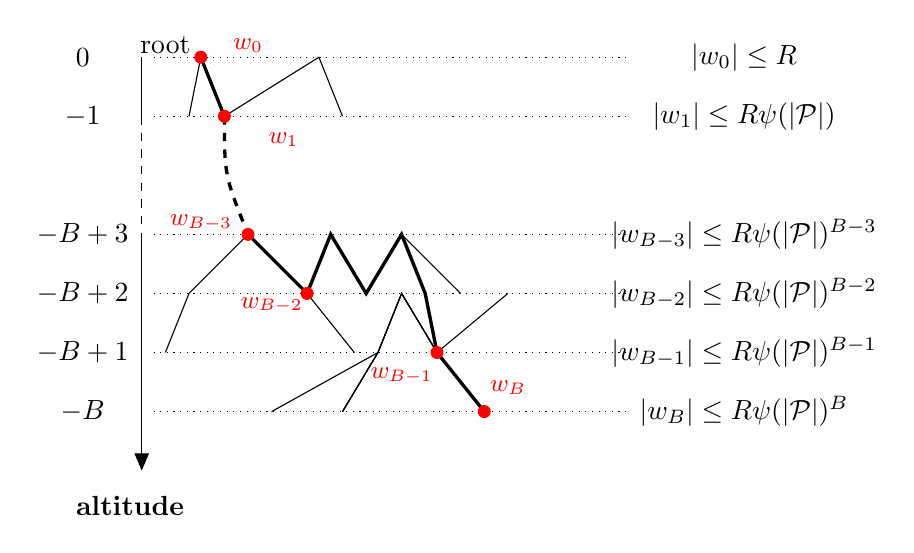
\begin{tikzpicture}[scale=1.5]
	
	\draw[dotted] (0,0.5) -- (4,0.5);
	\draw[dotted] (0,-0) -- (4,-0);
	\draw[dotted] (0,-1) -- (4,-1);
	\draw[dotted] (0,-1.5) -- (4,-1.5);
	\draw[dotted] (0,-2) -- (4,-2);
	\draw[dotted] (0,-2.5) -- (4,-2.5);
	
	\node at (-0.6,0.5) {$0$};
	\node at (-0.6,-0) {$-1$};
	\node at (-0.6,-1) {$-B+3$};
	\node at (-0.6,-1.5) {$-B+2$};
	\node at (-0.6,-2) {$-B+1$};
	\node at (-0.6,-2.5) {$-B$};
	
	\onslide<4->
	{
		\node at (5,0.5) {$|w_0| \leq R$};
	}
	
	\onslide<5->
	{
		\node at (5,-2) {$|w_{B-1}| \leq R\psi(|\mathcal{P}|)^{B-1}$};
		\node at (5,-1.5) {$|w_{B-2}|  \leq R\psi(|\mathcal{P}|)^{B-2}$};
		\node at (5,-1) {$|w_{B-3}| \leq R\psi(|\mathcal{P}|)^{B-3}$};
		\node at (5,0) {$|w_{1}| \leq R\psi(|\mathcal{P}|)$};
		\node at (5,-2.5) {$|w_B| \leq R\psi(|\mathcal{P}|)^{B}$};	
	}
	
	
	
	\draw (0.4,0.5) -- (0.6, 0);
	\draw (0.8, -1)  -- (1.3, -1.5) -- (1.5, -1) -- (1.8, -1.5) -- (2.1, -1) -- (2.3, -1.5) -- (2.4, -2) -- (2.8, -2.5);
	\draw (0.6, 0) -- (1.4, 0.5) -- (1.6, 0);
	\draw (2.1, -1) -- (2.6, -1.5);
	\draw (1.3, -1.5) -- (1.7,-2);
	\draw (0.8, -1) --  (0.3, -1.5) -- (0.1,-2);
	\draw (2.4, -2) -- (2.1, -1.5) -- (1.9, -2) -- (1.6, -2.5);
	\draw (2.4, -2) -- (2.1, -1.5) -- (1.9, -2) -- (1.6, -2.5);
	\draw (2.4, -2) -- (2.1, -1.5) -- (1.9, -2) -- (1.6, -2.5);
	\draw (2.4, -2) -- (3, -1.5);
	\draw (1.9, -2) -- (1, -2.5);
	\draw (0.4, 0.5) -- (0.3, 0);
	
	
	\onslide<2->
	{
		\draw[dashed, very thick] (0.6, 0) .. controls +(0,-0.5) and +(-0.2,0.5) .. (0.8, -1);  
		
		\draw[very thick] (0.4,0.5) -- (0.6, 0);
		\draw[very thick] (0.8, -1)  -- (1.3, -1.5) -- (1.5, -1) -- (1.8, -1.5) -- (2.1, -1) -- (2.3, -1.5) -- (2.4, -2) -- (2.8, -2.5);
	}
	
	\draw[->, >=triangle 45] (-0.1, -1) -- (-0.1, -3);
	\draw[, dashed] (-0.1, 0) -- (-0.1, -1);
	\draw (-0.1, 0.5) -- (-0.1, 0);
	
	\node (H) at (-0.2, -3.3) {$\mathbf{altitude}$};
	
	
		\node (R) at (0.1,0.6) {root};
	%	\node (AM) at (3,2.7) {$max alt$};
	\onslide<3->
	{
		\draw[red, fill=red] (0.4, 0.5) circle (0.05);
		\draw[red, fill=red] (0.6, 0) circle (0.05);
		\draw[red, fill=red] (0.8, -1) circle (0.05);
		\draw[red, fill=red] (1.3, -1.5) circle (0.05);
		\draw[red, fill=red] (2.4, -2) circle (0.05);
		\draw[red, fill=red] (2.8, -2.5) circle (0.05);
	}	
	\onslide<3->
	{
		\node[red] at (0.8, 0.6) {\small $w_0$};
		\node[red] at (1.1, -0.2) {\small $w_{1}$};
		\node[red] at (0.4, -0.9) {\small $w_{B-3}$};
		\node[red] at (1, -1.6) {\small $w_{B-2}$};
		\node[red] at (2.1, -2.2) {\small $w_{B-1}$};
		\node[red] at (3, -2.3) {\small $w_B$};
	}
	%	
	%	\node (txt) at (9.2, 2.7) {We consider a branch reaching $\altmax$. For all $i$,};
	%	\node (txt) at (8.9, 2.2) {let $w_i = \followlabelword{\node'_i}\#\followlabelmessage{\node'_i}$ where $\node'_i$ is the first};
	%	\node (txt) at (8.5, 1.7) {"follower node" at altitude $\altmax - i+1$.};
	%	
	%	\node (txt) at (9.45, 1) {Lemma~\ref{lem:bound-length-at-height-h} bounds the length of $w_i$ by $f_0(i)+2$, which};
	%	\node (txt) at (9.2, 0.5) {allows us to bound the number of red dots using};
	%	\node (txt) at (8.95, 0) {Lemma~\ref{lem:shortening-branches} and the "Length function theorem".};
\end{tikzpicture}
\end{frame}

% \begin{frame}{Bounding the tree}
	
% 	\begin{columns}
% 		\begin{column}{0.5\textwidth}
% 			We have bounds on:
			
% 			\begin{itemize}
% 				\item the maximal altitude
				
% 				\item the minimal altitude
				
% 				\item the size of nodes
% 			\end{itemize}
% 		\end{column}
		
% 		\begin{column}{0.5\textwidth}
% 			\pause
% 			We can infer bounds on 
			
% 			\begin{itemize}
% 				\item The length of branches
				
% 				\item The number of children of nodes
				
% 				\item The tree
% 			\end{itemize}
			
% 		\end{column}
% 	\end{columns}
	
% 	\end{frame}

\begin{frame}{Decidability}
	
	We have obtained bounds of the height of our witness trees; from there, we can easily bound the space needed to store such trees.
	
	\pause
	We can simply enumerate witness trees, thus
	
	\begin{block}{Theorem}
		{\COVER} for BNRA is decidable (and in class $\mathbf{F}_{\omega^\omega}$).
	\end{block}
	
	\pause
	
	By contrast,
	
	\begin{block}{Theorem}
		{\TARGET} is undecidable for BNRA.
	\end{block}
\end{frame}

\section{Complexity lower bound}

\begin{frame}{A matching lower bound}
		\begin{block}{Theorem}
		{\COVER} in BNRA is $\mathbf{F}_{\omega^\omega}$-hard, even in signature protocols with two registers per agent.
	\end{block}

	\pause 
	We proceed by reduction from \emph{lossy channel systems}: 
	
	\begin{block}{Theorem\footnotemark}
		Lossy channel system reachability is $\mathbf{F}_{\omega^\omega}$-hard.
	\end{block}

	\footnotetext<2->{Schnoebelen, Information Processing Letters '08}
\end{frame}


\begin{frame}{Lossy Channel Systems}
	Lossy Channel System = Transition system with FIFO memory + unreliable writes.
	
	\begin{center}
	\resizebox{!}{4.5cm}{
	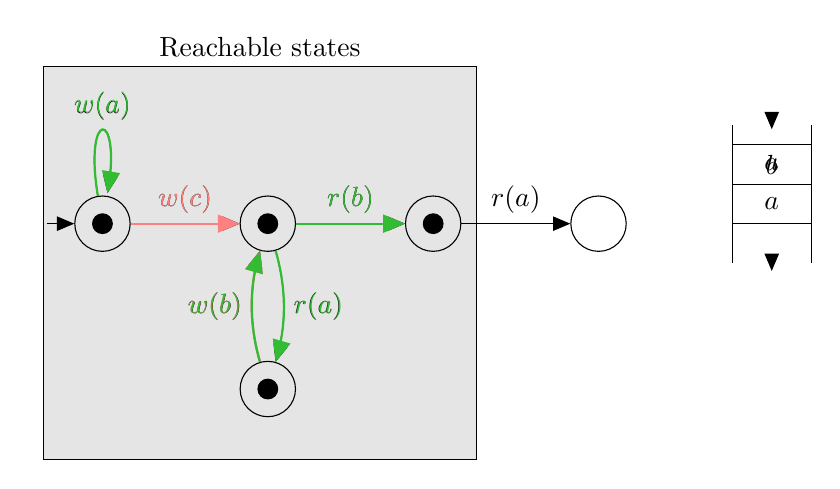
\begin{tikzpicture}[xscale=0.5,node distance=2.1cm,auto, AUT style,>= triangle
	45]
	\tikzstyle{initial}= [initial by arrow,initial text=,initial
	distance=.7cm]
	%	\tikzstyle{accepting}= [accepting by arrow,accepting text=,accepting
	%	distance=.7cm,accepting where =right]
	
	
	\onslide<10> {\draw[fill=gray!20] (-1.5, -3) rectangle (9.5, 2);
		\node (d) at (4,2.25) {Reachable states};
	}
	
	
	\node[state, initial, minimum width=0.1pt] (0) at (0,0) {};
	\node[state] [right of=0] (x) {};
	\node[state] [right of=x] (y) {};
	\node[state] [right of=y] (z) {};
	\node[state] [below of=x] (t) {};
	
	
	%	\path[->, bend left=10] 	
	%	(y) edge node[above] {$\mathbf{br}(b)$} (x)
	%	;
	
	\onslide<1,4-10>{\path[loop above] (0) edge node[above] {$w(a)$} (0);}
	\onslide<2-3>{\path[loop above,thick, color=RealGreen] (0) edge node[above] {\color{RealGreen}\textbf{$w(a)$}} (0);}
	
	\onslide<1-8,10>{\path[->] (x) edge node[above] {$r(b)$} (y);}
	\onslide<9>{\path[->, thick, color=RealGreen] (x) edge node[above] {\color{RealGreen}\textbf{$r(b)$}} (y);}
	
	\onslide<1-3,5-10>{\path[->] (0) edge node[above] {$w(c)$} (x);}
	\onslide<4>{\path[->, thick, color=red!50] (0) edge node[above] {\color{red!50}\textbf{$w(c)$}} (x);}
	
	\path[->] (y) edge node[above] {$r(a)$} (z);
	
	
	\onslide<1-4,6,8-10>{\path[->, bend left] (x) edge node[right] {$r(a)$} (t);}
	\onslide<5,7>{\path[->, bend left,thick, color=RealGreen] (x) edge node[right] {\color{RealGreen}\textbf{$r(a)$}} (t);}
	
	\onslide<1-5,7,9-10>{\path[->, bend left] (t) edge node[left] {$w(b)$} (x);}
	\onslide<6>{\path[->, bend left,thick, color=red!50] (t) edge node[left] {\color{red!50}\textbf{$w(b)$}} (x);}
	\onslide<8>{\path[->, bend left,thick, color=RealGreen] (t) edge node[left] {\color{RealGreen}\textbf{$w(b)$}} (x);}
	
	
	
	\onslide<3-4>
	{
	\draw (16,0) rectangle (18,0.5);
	\node at (17,0.25) {$a$};
}
	\onslide<2-6,8>
	{
	\draw (16,0.5) rectangle (18,1);
}
\onslide<2-6>
{
	\node at (17, 0.75) {$a$};
}
\onslide<8>
{
	\node at (17, 0.75) {$b$};
}


\onslide<1-3>
{
	\draw[fill=black] (0,0) ellipse (0.25 and 0.125);
}

\onslide<4,6,8>
{
	\draw[fill=black] (4.2,0) ellipse (0.25 and 0.125);
}

\onslide<5,7>
{
	\draw[fill=black] (4.2,-2.1) ellipse (0.25 and 0.125);
}

\onslide<9>
{
	\draw[fill=black] (8.4,0) ellipse (0.25 and 0.125);
}

\draw (16,-0.5) -- (16, 1.25);
\draw (18,-0.5) -- (18, 1.25);

\draw[->] (17, -0.4) -- (17, -0.6);
\draw[->] (17, 1.4) -- (17, 1.2);


\end{tikzpicture}
	}
	\end{center}

	\onslide<11-> Lossy channel system reachability asks if one can reach a given state. This problem is decidable but has very high complexity: it is $\mathbf{F}_{\omega^\omega}$-complete. 
\end{frame}


\begin{frame}{Encoding Lossy Channel Systems in BNRA}
	We simulate a lossy channel system through a chain of agents that each apply a transition.
	
	Each agent stores:
	\begin{itemize}
		\item An identifier for itself
		
		\item Its predecessor's identifier
	\end{itemize} 
	
	\centering
	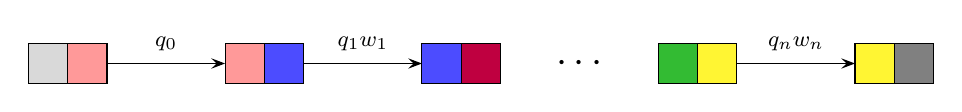
\begin{tikzpicture}

\draw[white, fill=gray!30] (0,0) rectangle (0.5,0.5);
\draw[white, fill=red!40] (2.5,0) rectangle (3,0.5);
\draw[white, fill=blue!70] (5,0) rectangle (5.5,0.5);
\draw[white, fill=RealGreen] (8,0) rectangle (8.5,0.5);
\draw[white, fill=yellow!80] (10.5,0) rectangle (11,0.5);

\draw[white, fill=red!40] (0.5,0) rectangle (1,0.5);
	\draw[white, fill=blue!70] (3,0) rectangle (3.5,0.5);
\draw[white, fill=purple] (5.5,0) rectangle (6,0.5);
\draw[white, fill=yellow!80] (8.5,0) rectangle (9,0.5);
\draw[white, fill=gray] (11,0) rectangle (11.5,0.5);
	
\draw (0,0) rectangle (1,0.5);
\draw (2.5,0) rectangle (3.5,0.5);
\draw (5,0) rectangle (6,0.5);
\draw (8,0) rectangle (9,0.5);
\draw (10.5,0) rectangle (11.5,0.5);

\draw (0.5,0) -- (0.5,0.5);
\draw (3,0) -- (3,0.5);
\draw (5.5,0) -- (5.5,0.5);
\draw (8.5,0) -- (8.5,0.5);
\draw (11,0) -- (11,0.5);


\draw[->, arrows = {-Stealth[length=5pt, inset=2pt]}] (1,0.25) -- (2.5,0.25);
\draw[->, arrows = {-Stealth[length=5pt, inset=2pt]}] (3.5,0.25) -- (5,0.25);
\draw[->, arrows = {-Stealth[length=5pt, inset=2pt]}] (9,0.25) -- (10.5,0.25);
	
\node (D) at (7,0.25) {\Large$\cdots$};

\node (X) at (1.75,0.5) {\footnotesize $q_0$};
\node (Y) at (4.25,0.5) {\footnotesize $q_1 w_1$};
\node (Z) at (9.75,0.5) {\footnotesize $q_{n} w_{n}$};
\end{tikzpicture}
	
\end{frame}


\begin{frame}{Encoding write transitions of Lossy Channel Systems}
	\centering
	\begin{tikzpicture}[node distance=2.8cm,auto, AUT style,>= triangle
	45]
	\tikzstyle{initial}= [initial by arrow,initial text=,initial
	distance=.7cm]
	%	\tikzstyle{accepting}= [accepting by arrow,accepting text=,accepting
	%	distance=.7cm,accepting where =right]
	\tikzset{every node/.style ={font = \small}}
	
	\node[state, initial, minimum width=0.1pt] (0) at (0,0) {};
	\node[state] [right of=0] (l1) {};
	\node[state] [right of=l1] (l2) {};
	\node[state] [below = 0.8 of 0] (t1) {};
	\node[state] [below = 0.8 of t1] (t2) {};
	\node[state] [below = 0.8 of t2] (echo) {};
	\node[state] [right of=t2] (t3) {};
	\node[state] [right of = t3] (t4) {};
	\node[state] [below = 0.8 of t4] (t5) {};
	

	\path[->] (0) edge node[above] {$\mathbf{br}(q_0, \reg_1)$} (l1);
	\path[->] (l1) edge node[above] {$\mathbf{br}(\mathsf{end}, \reg_1)$} (l2);
	
	\path[->] (0) edge node[left] {$\mathbf{rec}(q, \downarrow\reg_2)$} (t1);
	\path[->] (t1) edge node[left] {$\mathbf{br}(q', \reg_1)$} (t2);
	\path[->] (t2) edge node[above] {$\mathbf{rec}(\mathsf{end}, =\reg_2)$} (t3);
	\path[->, bend right=20] (t2) edge node[left] {$\mathbf{rec}(x, =\reg_2)$} (echo);
	\path[->, bend right=20] (echo) edge node[right] {$\mathbf{br}(x, \reg_1)$} (t2);
	\path[->] (t3) edge node[above] {$\mathbf{br}(\texttt{a}, \reg_1)$} (t4);
	\path[->] (t4) edge node[right] {$\mathbf{br}(\mathsf{end}, \reg_1)$} (t5);

	\draw (-2.3,-5.2) rectangle (7.5, -0.45);
	\node (d) at (2.6,-5.7) {Gadget for a transition $q \xrightarrow{\mathsf{write}(\texttt{a})} q'$ of the LCS};
\end{tikzpicture}

\end{frame}

\begin{frame}{Encoding read transitions of Lossy Channel Systems}
	\centering
	\begin{tikzpicture}[node distance=2.8cm,auto, AUT style,>= triangle
	45]
	\tikzstyle{initial}= [initial by arrow,initial text=,initial
	distance=.7cm]
	%	\tikzstyle{accepting}= [accepting by arrow,accepting text=,accepting
	%	distance=.7cm,accepting where =right]
	\tikzset{every node/.style ={font = \small}}
	
	\node[state, initial, minimum width=0.1pt] (0) at (0,0) {};
	\node[state] [right of=0] (l1) {};
	% \node[state] [right of=l1] (l2) {};
	\node[state] [below = 0.8 of 0] (t1) {};
	\node[state] [below = 0.8 of t1] (t2) {};
	\node[state] [below = 0.8 of t3] (echo) {};
	\node[state] [right of=t2] (t3) {};
	% \node[state] [right of = t3] (t4) {};
	% \node[state] [below = 0.8 of t4] (t5) {};
	

	\path[->] (0) edge node[above] {$\mathbf{br}(q_0, \reg_1)$} (l1);
	% \path[->] (l1) edge node[above] {$\mathbf{br}(\mathsf{end}, \reg_1)$} (l2);
	
	\path[->] (0) edge node[left] {$\mathbf{rec}(q, \downarrow\reg_2)$} (t1);
	\path[->] (t1) edge node[left] {$\mathbf{br}(q', \reg_1)$} (t2);
	\path[->] (t2) edge node[above] {$\mathbf{rec}(\texttt{a}, =\reg_2)$} (t3);
	\path[->, bend right=20] (t3) edge node[left] {$\mathbf{rec}(x, =\reg_2)$} (echo);
	\path[->, bend right=20] (echo) edge node[right] {$\mathbf{br}(x, \reg_1)$} (t3);
	% \path[->] (t3) edge node[above] {$\mathbf{rec}(\mathsf{end}, =\reg_2)$} (t4);
	% \path[->] (t4) edge node[right] {$\mathbf{br}(\mathsf{end}, \reg_1)$} (t5);

	\draw (-2.3,-5.2) rectangle (5, -0.45);
	\node[minimum width = 5cm] (d) at (1.5,-5.7) {Gadget for a transition $q \xrightarrow{\mathsf{read}(\texttt{a})} q'$ of the lossy channel system};
\end{tikzpicture} 
\end{frame}

\begin{frame}{Summary of complexity results}

	\begin{block}{Theorem}
		{\COVER} in BNRA is $\mathbf{F}_{\omega^\omega}$-complete.
	\end{block}
		
	\pause
	\begin{block}{Theorem}
	\COVER{} for BNRA with one register per agent is NP-complete. 
	\end{block}
\end{frame}

\begin{frame}{}
	
	\Huge \textbf{Thank you for your attention!}
	
\end{frame}

\appendix
\begin{frame}
\end{frame}


\begin{frame}{Turning the communication graph into a tree}
\centering
 	\definecolor{colorA}{rgb}{0.93, 0.53, 0.18}
    \definecolor{colorB}{rgb}{0.54, 0.81, 0.94}
    \definecolor{colorC}{rgb}{0.01, 0.75, 0.24}
    \definecolor{stepcolor}{rgb}{0.8, 0.25, 0.33}
\begin{tikzpicture}[auto]
\tikzstyle{agent} = [rectangle, draw, minimum size = 1cm]
\tikzstyle{symbol} = [draw = none, color = black]
\tikzstyle{stepnumber} = [circle, draw = stepcolor, minimum size = 0.2cm, inner sep = 1pt, color = stepcolor]
\tikzstyle{sendto} = [-latex]
\fill[colorA!50] (-3,1.5) .. controls (2.5,1.5) and (2.5,-1.5) .. (-3,-1.5) -- (-3,1.5);
\fill[colorB!50] (8,3.5) .. controls (2.5,3.5) and (2.5,0.5) .. (8,0.5) -- (8,3.5);
\fill[colorC!50] (8,-0.5) .. controls (2.5,-0.5) and (2.5,-3.5) .. (8,-3.5) -- (8,-0.5);

\node[agent] at (0,0) (A) {$A$};
\node[agent] at (5, 2) (B) {$B$};
\node[agent] at (5, -2) (C) {$C$};

\onslide<2->
\node at (5,3.5) (qf) {$q_f$};
\draw[sendto, bend left = 25] (A) to[bend left = 40] node[above, pos = 0.5, symbol] {\texttt{a}} node[below,  stepnumber, yshift = -0.1cm] {$1$} (B); 
\draw[sendto] (A) to node[above, pos = 0.5, symbol] {\texttt{a}} node[below, stepnumber, yshift = -0.1cm] {$1$} (C); 
\onslide<3->
\draw[sendto] (C) to[bend left = 40] node[above, pos = 0.5, symbol] {\texttt{b}} node[below, stepnumber] {$2$} (A); 
\onslide<4->
\draw[sendto] (B) to node[above, pos = 0.5, symbol] {\texttt{c}} node[below, stepnumber, yshift = -0.1cm] {$3$} (A); 
\onslide<5->
\draw[sendto] (A) to[bend right = 40] node[above, pos = 0.5, symbol] {\texttt{d}} node[below,  stepnumber] {$4$}  (B); \
\onslide<6->
\draw[sendto, decorate, decoration = snake] (B) to node[right,  stepnumber, xshift = 0.1cm] {$5$} (qf);

\onslide<7->
\node[align = center] at ($(A)-(1.5,0)$) {Tasks: \\ $\epsilon \mapsto \texttt{a}$ \\ $\texttt{b}, \texttt{c} \mapsto \texttt{a} \texttt{d}$};
\node[align = center] at ($(B)+(1.5,0)$) {Tasks: \\ $\texttt{a} \mapsto \texttt{c}$ \\$\texttt{a} \texttt{d} \mapsto q_f$};
\node[font = \tiny, align = center] at ($(B)+(1.5,-1.0)$) {$\texttt{a} \texttt{d}$ = receive $\texttt{a}$ then $\texttt{d}$ \\ \emph{with same} value};
\node[align = center] at ($(C)+(1.5,0)$) {Tasks: \\ $\texttt{a} \mapsto \texttt{b}$};

\end{tikzpicture}
\end{frame}

\begin{frame}{Turning the communication graph into a tree}
\begin{minipage}{0.55\linewidth}
\centering
\resizebox{6.5cm}{!}{
 	\definecolor{colorA}{rgb}{0.93, 0.53, 0.18}
    \definecolor{colorB}{rgb}{0.54, 0.81, 0.94}
    \definecolor{colorC}{rgb}{0.01, 0.75, 0.24}
    \definecolor{stepcolor}{rgb}{0.8, 0.25, 0.33}
\begin{tikzpicture}
\tikzstyle{agent} = [rectangle, draw, minimum size = 1cm]
\tikzstyle{symbol} = [draw = none, color = black]
\tikzstyle{stepnumber} = [circle, draw = stepcolor, minimum size = 0.2cm, inner sep = 1pt, color = stepcolor]
\tikzstyle{sendto} = [-latex]
\fill[colorA!50] (-3,1.5) .. controls (2.5,1.5) and (2.5,-1.5) .. (-3,-1.5) -- (-3,1.5);
\fill[colorB!50] (8,3.5) .. controls (2.5,3.5) and (2.5,0.5) .. (8,0.5) -- (8,3.5);
\fill[colorC!50] (8,-0.5) .. controls (2.5,-0.5) and (2.5,-3.5) .. (8,-3.5) -- (8,-0.5);

\node[agent] at (0,0) (A) {$A$};
\node[agent] at (5, 2) (B) {$B$};
\node[agent] at (5, -2) (C) {$C$};

\node at (5,3.5) (qf) {$q_f$};
\draw[sendto, bend left = 25] (A) to[bend left = 40] node[above, pos = 0.5, symbol] {\texttt{a}} node[below,  stepnumber, yshift = -0.1cm] {$1$} (B); 
\draw[sendto] (A) to node[above, pos = 0.5, symbol] {\texttt{a}} node[below, stepnumber, yshift = -0.1cm] {$1$} (C); 
\draw[sendto] (C) to[bend left = 40] node[above, pos = 0.5, symbol] {\texttt{b}} node[below, stepnumber] {$2$} (A); 
\draw[sendto] (B) to node[above, pos = 0.5, symbol] {\texttt{c}} node[below, stepnumber, yshift = -0.1cm] {$3$} (A); 
\draw[sendto] (A) to[bend right = 40] node[above, pos = 0.5, symbol] {\texttt{d}} node[below,  stepnumber] {$4$}  (B); 
\draw[sendto, decorate, decoration = snake] (B) to node[right,  stepnumber, xshift = 0.1cm] {$5$} (qf);

\node[align = center] at ($(A)-(1.5,0)$) {Tasks: \\ $\epsilon \mapsto \texttt{a}$ \\ $\texttt{b}, \texttt{c} \mapsto \texttt{a} \texttt{d}$};
\node[align = center] at ($(B)+(1.5,0)$) {Tasks: \\ $\texttt{a} \mapsto \texttt{c}$ \\$\texttt{a} \texttt{d} \mapsto q_f$};
\node[align = center] at ($(C)+(1.5,0)$) {Tasks: \\ $\texttt{a} \mapsto \texttt{b}$};

\end{tikzpicture}
}
\end{minipage}
\begin{minipage}{0.1\linewidth}
$\longrightarrow$
\end{minipage}
\begin{minipage}{0.25 \linewidth}
\resizebox{!}{5cm}{
\definecolor{colorA}{rgb}{0.93, 0.53, 0.18}
\definecolor{colorB}{rgb}{0.54, 0.81, 0.94}
\definecolor{colorC}{rgb}{0.01, 0.75, 0.24}
\begin{tikzpicture}
\tikzstyle{agent} = [rectangle, draw, minimum size = 1cm]
\tikzstyle{symbol} = [draw = none, color = black]
\node[agent, fill = colorA!50] at (0,0) (A2) {$A$};
\node[agent, fill = colorB!50] at (0,-2) (B1) {$B$};
\node[agent, fill = colorA!50] at (-4,-4) (A3) {$A$};
\node[agent, fill = colorC!50] at (-2,-4) (C2) {$C$};
\node[agent, fill = colorA!50] at (0,-4) (A4) {$A$};
\node[agent, fill = colorB!50] at (0,-6) (B2) {$B$};
\node at (0,-7.5) (qf) {$q_f$};
\draw[-latex] (A2) to node[right, symbol] {$\texttt{a}$} (B1); 
\draw[-latex] (B1) to node[right, symbol] {$\texttt{c}$} (A4); 
\draw[-latex] (A3) to node[above, symbol] {$\texttt{a}$} (C2); 
\draw[-latex] (C2) to node[above, symbol] {$\texttt{b}$} (A4); 
\draw[-latex] (A4) to node[right, symbol] {$\texttt{a} \texttt{d}$} (B2); 
\draw[-latex, decorate, decoration = snake] (B2) to (qf); 
\end{tikzpicture}
}
\end{minipage}
\hfill
\end{frame}

\end{document}